% !TeX program = lualatex
\documentclass[a4paper,twoside,11pt]{report} %openright
\newcommand{\documenttype}{Master Thesis}
\newcommand{\thesistitle}{3D human interaction synthesis for action recognition data augmentation}
\newcommand{\thesissubtitle}{}

\newcommand{\thesisauthor}{Anders Bredgaard Thuesen} % Your name :) 
\newcommand{\studentnumber}{s183926}
\newcommand{\thedate}{June, 2024} % For example "June, 2019"

\newcommand{\department}{DTU Compute}
\newcommand{\departmentdescriber}{Department of Applied Mathematics and Computer Science}
\newcommand{\addressI}{Richard Petersens Plads, Building 324}
\newcommand{\addressII}{2800 Kgs. Lyngby}
\newcommand{\departmentwebsite}{www.compute.dtu.dk}

%\usepackage{microtype}      % better looking text
%\usepackage[utf8]{inputenc}
\usepackage{fontspec}       % Package for custom fonts
\usepackage[]{geometry}     % Package for changing page margins (before fancyhdr) 
\usepackage{fancyhdr}       % Package to change header and footer
\usepackage{parskip}        % Package to tweak paragraph skipping (instead of indents a small skip is added after every paragraph)
\usepackage{titlesec}
\usepackage{tikz}           % Package for drawing
\usepackage{pgfplots}       % Package for creating graphs and charts
\usepackage{xcolor}         % Package for defining DTU colours to be used
\usepackage{amsmath}        % For aligning equations among other
\usepackage{siunitx}        % SI units
\usepackage{listings}       % Package for inserting code, (before cleveref)
\PassOptionsToPackage{hyphens}{url} % Ability to line break urls at hyphens
\usepackage{hyperref}       % Package for cross referencing (also loads url package)
\usepackage{cleveref}       % improved cross referencing
\usepackage{textcomp}       % \textdegree = °C and other useful symbols
\usepackage[english]{babel} % localisation 
\usepackage{caption}        % better captions
\usepackage{subcaption}     % for subfigures
\usepackage{csquotes}       % For biblatex with babel
\usepackage[backend=biber,style=authoryear,sorting=none]{biblatex} % Package for bibliography (citing)
\bibliography{bibliography.bib}
\usepackage{tabularx}       % for ability to adjust column spacing in tabular better
\usepackage{booktabs}       % for better tables
\usepackage{float}          % floating figures in correct places
\usepackage{calc}           % Adds ability for latex to calculate (3pt+2pt) 
% \usepackage[printwatermark=false]{xwatermark} % Package for wartermark. Toggle printwatermark true or false to include or remove the watermark
\usepackage{blindtext}
\usepackage{amsfonts}
\usepackage{bm}

% Define new commands
\newcommand{\norm}[2]{\left \lVert #1 \right \rVert_{#2}}
\newcommand{\vect}[1]{\boldsymbol{\mathbf{#1}}}

\DeclareMathOperator*{\argmax}{argmax\,}
\DeclareMathOperator*{\argmin}{argmin\,}
% Colours! 
\newcommand{\targetcolourmodel}{cmyk} % rgb for a digital version, cmyk for a printed version. Only use lowercase
\selectcolormodel{\targetcolourmodel}

% Define colours from https://www.designguide.dtu.dk/
\definecolor{dtured}    {rgb/cmyk}{0.6,0,0 / 0,0.91,0.72,0.23}
\definecolor{blue}      {rgb/cmyk}{0.1843,0.2431,0.9176 / 0.88,0.76,0,0}
\definecolor{brightgreen}{rgb/cmyk}{0.1216,0.8157,0.5098 / 0.69,0,0.66,0}
\definecolor{navyblue}  {rgb/cmyk}{0.0118,0.0588,0.3098 / 1,0.9,0,0.6}
\definecolor{yellow}    {rgb/cmyk}{0.9647,0.8157,0.3019 / 0.05,0.17,0.82,0}
\definecolor{orange}    {rgb/cmyk}{0.9882,0.4627,0.2039 / 0,0.65,0.86,0}
\definecolor{pink}      {rgb/cmyk}{0.9686,0.7333,0.6941 / 0,0.35,0.26,0}
\definecolor{grey}      {rgb/cmyk}{0.8549,0.8549,0.8549 / 0,0,0,0.2}
\definecolor{red}       {rgb/cmyk}{0.9098,0.2471,0.2824 / 0,0.86,0.65,0}
\definecolor{green}     {rgb/cmyk}{0,0.5333,0.2078 / 0.89,0.05,1,0.17}
\definecolor{purple}    {rgb/cmyk}{0.4745,0.1373,0.5569 / 0.67,0.96,0,0}

\newcommand{\dtulogocolour}{white} % Colour of the DTU logo: white, black or dtured
\newcommand{\frontpagetextcolour}{white} % front page text colour: white or black
\colorlet{frontbackcolor}{blue} % Set the background colour of the front- and back page. Choose the colour so it matches the main colour of front page picture

% DTU colours for diagrams
% You might want to make the front/back page background colour the first colour in the plot cycle list.
\pgfplotscreateplotcyclelist{DTU}{%
dtured,         fill=dtured,        \\%
blue,           fill=blue,          \\%
brightgreen,    fill=brightgreen    \\%
navyblue,       fill=navyblue       \\%
yellow,         fill=yellow         \\%
orange,         fill=orange         \\%
grey,           fill=grey           \\%
red,            fill=red            \\%
green,          fill=green          \\%
purple,         fill=purple         \\%
}


% Font
% There is no corporate serif font in the DTU design guide. The DTU design team has proposed to use Neo Sans for headings - and Arial for the body text.
% To change heading font to NeoSans Pro please upload both NeoSansPro-Regular.otf and NeoSansPro-Medium.otf to the root directory.
\setmainfont{Arial}
\renewcommand\thepart{Part \Roman{part}}
\IfFontExistsTF{NeoSansPro-Medium.otf}
{ %If True set headings to NeoSans Pro
\newfontface\NeoSansProReg{NeoSansPro-Regular.otf}
\newfontface\NeoSansProMed{NeoSansPro-Medium.otf}
\titleformat{\part}[display]{\NeoSansProMed \huge \centering}{\NeoSansProMed \Huge \thepart}{1em}{\thispagestyle{empty}}{}
\titleformat{\chapter}{\NeoSansProMed\huge}{\thechapter}{1em}{\raggedright}
\titleformat{\section}{\NeoSansProMed\Large}{\thesection}{1em}{\raggedright}
\titleformat{\subsection}{\NeoSansProMed\large}{\thesubsection}{1em}{\raggedright}
\titleformat{\subsubsection}{\NeoSansProMed\normalsize}{\thesubsubsection}{1em}{\raggedright}
\newcommand\TitleFont[1]{{\NeoSansProMed #1}}
\newcommand\titlefont[1]{{\NeoSansProReg #1}}
}
{ % If false
\titleformat{\part}[display]{\bfseries\huge \centering}{\bfseries\Huge \thepart}{1em}{\thispagestyle{empty}}{}
\titleformat{\chapter}{\bfseries\huge}{\thechapter}{1em}{\raggedright}
\titleformat{\section}{\bfseries\Large}{\thesection}{1em}{\raggedright}
\titleformat{\subsection}{\bfseries\large}{\thesubsection}{1em}{\raggedright}
\titleformat{\subsubsection}{\bfseries\normalsize}{\thesubsubsection}{1em}{\raggedright}
\newcommand\TitleFont[1]{{\bfseries #1}}
\newcommand\titlefont[1]{{#1}}
}
\urlstyle{sf}
%\def\UrlFont{\NeoSansProReg}


% If you wish to use the pdflatex compiler, sans-serif Helvetica can be used as a replacement for Arial. In this way you will be able to use the microtype package. Remember to add \usepackage[utf8]{inputenc} and disable the fontspec package. 
%\newcommand\TitleFont[1]{{\bfseries #1}}
%\newcommand\titlefont[1]{{#1}}
%\fontfamily{qhv}\selectfont
%\renewcommand{\familydefault}{\sfdefault}


% Watermark for confidential or draft (or anything else)
%\sffamily % set the correct font for the watermark
%%\newsavebox\mybox
%%\savebox\mybox{\tikz[color=grey,opacity=0.5]\node{Template};}

%%\newwatermark*[
%%  oddpages,
%%  angle=60,
%%  scale=12,
%%  %fontfamily=qhv,
%%  xpos=-40,
%%  ypos=30,
%%]{\usebox\mybox}

%%\newwatermark*[
%%  evenpages,
%%  angle=60,
%%  scale=12,
%%  %fontfamily=qhv,
%%  xpos=-50,
%%  ypos=30,
%%]{\usebox\mybox}


% Table of contents (TOC) and numbering of headings
\setcounter{tocdepth}{2}    % Depth of table of content: sub sections will not be included in table of contents
\setcounter{secnumdepth}{2} % Depth of section numbering: sub sub sections are not numbered

\makeatletter % Reset chapter numbering for each part
\@addtoreset{chapter}{part}
\makeatother  

% Spacing of titles and captions
\titlespacing\chapter{0pt}{0pt plus 4pt minus 2pt}{4pt plus 2pt minus 2pt}
\titlespacing\section{0pt}{12pt plus 3pt minus 3pt}{2pt plus 1pt minus 1pt}
\titlespacing\subsection{0pt}{8pt plus 2pt minus 2pt}{0pt plus 1pt minus 1pt}
\titlespacing\subsubsection{0pt}{4pt plus 1pt minus 1pt}{-2pt plus 1pt minus 1pt}
\captionsetup{belowskip=\parskip,aboveskip=4pt plus 1pt minus 1pt}

% Setup header and footer
\fancypagestyle{main}{% All normal pages
    \fancyhead{}
    \fancyfoot{}
    \renewcommand{\headrulewidth}{0pt}
    \fancyfoot[LE,RO]{\footnotesize \thepage}
    \fancyfoot[RE,LO]{\footnotesize \thesistitle} % - \rightmark
    \fancyhfoffset[E,O]{0pt}
}
\fancypagestyle{plain}{% Chapter pages
    \fancyhead{}
    \fancyfoot{}
    \renewcommand{\headrulewidth}{0pt}
    \fancyfoot[LE,RO]{\footnotesize \thepage}
    \fancyfoot[RE,LO]{\footnotesize \thesistitle} % - \leftmark
    \fancyhfoffset[E,O]{0pt}
}


% Setup for diagrams and graphs (tikz pictures) 
\usetikzlibrary{spy}    % For magnifying anything within a tikzpicture, see the line graph
\usepgfplotslibrary{statistics} % Package for the boxplot
\pgfplotsset{ % Setup for diagrams
compat=newest,
major x grid style={line width=0.5pt,draw=grey},
major y grid style={line width=0.5pt,draw=grey},
legend style={at={(0.5,-0.1)}, anchor=north,fill=none,draw=none,legend columns=-1,/tikz/every even column/.append style={column sep=10pt}},
axis line style={draw=none},
tick style={draw=none},
every axis/.append style={ultra thick},
tick label style={/pgf/number format/assume math mode}, % To apply main font to tick labels (numbers on the axis)
}
\tikzset{every mark/.append style={scale=1.5}}


% Hypersetup
\hypersetup{
    pdfauthor={\thesisauthor},
    pdftitle={\thesistitle},
    pdfsubject={\thesissubtitle},
    pdfdisplaydoctitle,
    bookmarksnumbered=true,
    bookmarksopen,
    breaklinks,
    linktoc=all,
    plainpages=false,
    unicode=true,
    colorlinks=false,
    hidelinks,                        % Do not show boxes or coloured links.
}


% Listings setup
\lstset{
    basicstyle=\footnotesize\ttfamily,% the size of the fonts that are used for the code
    commentstyle=\color{green},       % comment style
    keywordstyle=\bfseries\ttfamily\color{blue}, % keyword style
    numberstyle=\sffamily\tiny\color{grey}, % the style that is used for the line-numbers
    stringstyle=\color{purple},       % string literal style
    rulecolor=\color{grey},           % if not set, the frame-color may be changed on line-breaks within not-black text (e.g. comments (green here))
    breakatwhitespace=false,          % sets if automatic breaks should only happen at whitespace
    breaklines=true,                  % sets automatic line breaking
    captionpos=b,                     % sets the caption-position to bottom
    deletekeywords={},                % if you want to delete keywords from the given language
    escapeinside={\%*}{*)},           % if you want to add LaTeX within your code
    frame=single,                     % adds a frame around the code
    xleftmargin=4pt, 
    morekeywords={*,...},             % if you want to add more keywords to the set
    numbers=left,                     % where to put the line-numbers; possible values are (none, left, right)
    numbersep=10pt,                   % how far the line-numbers are from the code
    showspaces=false,                 % show spaces everywhere adding particular underscores; it overrides 'showstringspaces'
    showstringspaces=false,           % underline spaces within strings only
    showtabs=false,                   % show tabs within strings adding particular underscores
    stepnumber=1,                     % the step between two line-numbers. If it's 1, each line will be numbered
    tabsize=2,                        % sets default tabsize to 2 spaces
    title=\lstname,                   % show the filename of files included with \lstinputlisting; also try caption instead of title
}

% Signature field
\newlength{\myl}
\newcommand{\namesigdatehrule}[1]{\par\tikz \draw [black, densely dotted, very thick] (0.04,0) -- (#1,0);\par}
\newcommand{\namesigdate}[2][]{%
\settowidth{\myl}{#2}
\setlength{\myl}{\myl+10pt}
\begin{minipage}{\myl}%
\begin{center}
    #2  % Insert name from the command eg. \namesigdate{\authorname}
    \vspace{1.5cm} % Spacing between name and signature line 
    \namesigdatehrule{\myl}\smallskip % Signature line and a small skip
    \small \textit{Signature} % Text under the signature line "Signature"
    \vspace{1.0cm} % Spacing between "Signature" and the date line
    \namesigdatehrule{\myl}\smallskip % Date line and a small skip
    \small \textit{Date} % Text under date line "Date" 
\end{center}
\end{minipage}
}

% For the back page: cleartoleftpage
\newcommand*\cleartoleftpage{%
  \clearpage
  \ifodd\value{page}\hbox{}\newpage\fi
}


\setlength\bibitemsep{0.5\baselineskip}

\begin{document}

\pagenumbering{roman}
\title{\thesistitle} 
\author{\thesisauthor} 
\date{\thedate} 

\begin{titlepage}

\newgeometry{left=11mm,right=11mm,top=50mm,bottom=0pt}
\pagecolor{frontbackcolor}
\color{\frontpagetextcolour}

{ % Thesis title (to change see Setup/Settings.tex) 
\Huge
\begin{tabular}{p{\linewidth}}
\TitleFont{\thesistitle}   \\ 
\TitleFont{\thesissubtitle} \bigskip \\ 
\titlefont{\documenttype}
\end{tabular}
}

% DTU department (to change see Setup/Settings.tex) 
\begin{tikzpicture}[remember picture,overlay]
\node[anchor=north east, 
      xshift=-10mm, 
      yshift=-12mm] 
      at (current page.north east) 
      {
        \color{\frontpagetextcolour}
        \begin{tabular}{r} 
        \textbf{\department} \\ 
        \departmentdescriber
        \end{tabular}
      }; 
\end{tikzpicture}

% DTU logo
\begin{tikzpicture}[remember picture,overlay]
\node[anchor=north west, 
      xshift=8.9mm, 
      yshift=-8.3mm] 
     at (current page.north west) 
     {\includegraphics[width=14.75mm,keepaspectratio]{Pictures/Logos/\dtulogocolour_\targetcolourmodel.pdf}}; 
\end{tikzpicture}

% Cover photo
\begin{tikzpicture}[remember picture,overlay]
\node[anchor=south, % anchor is bottom of picture
      xshift=0pt, 
      yshift=-2.9mm] % shifting picture to actually be at the bottom of the page
     at (current page.south) % placement at bottom of the page
     {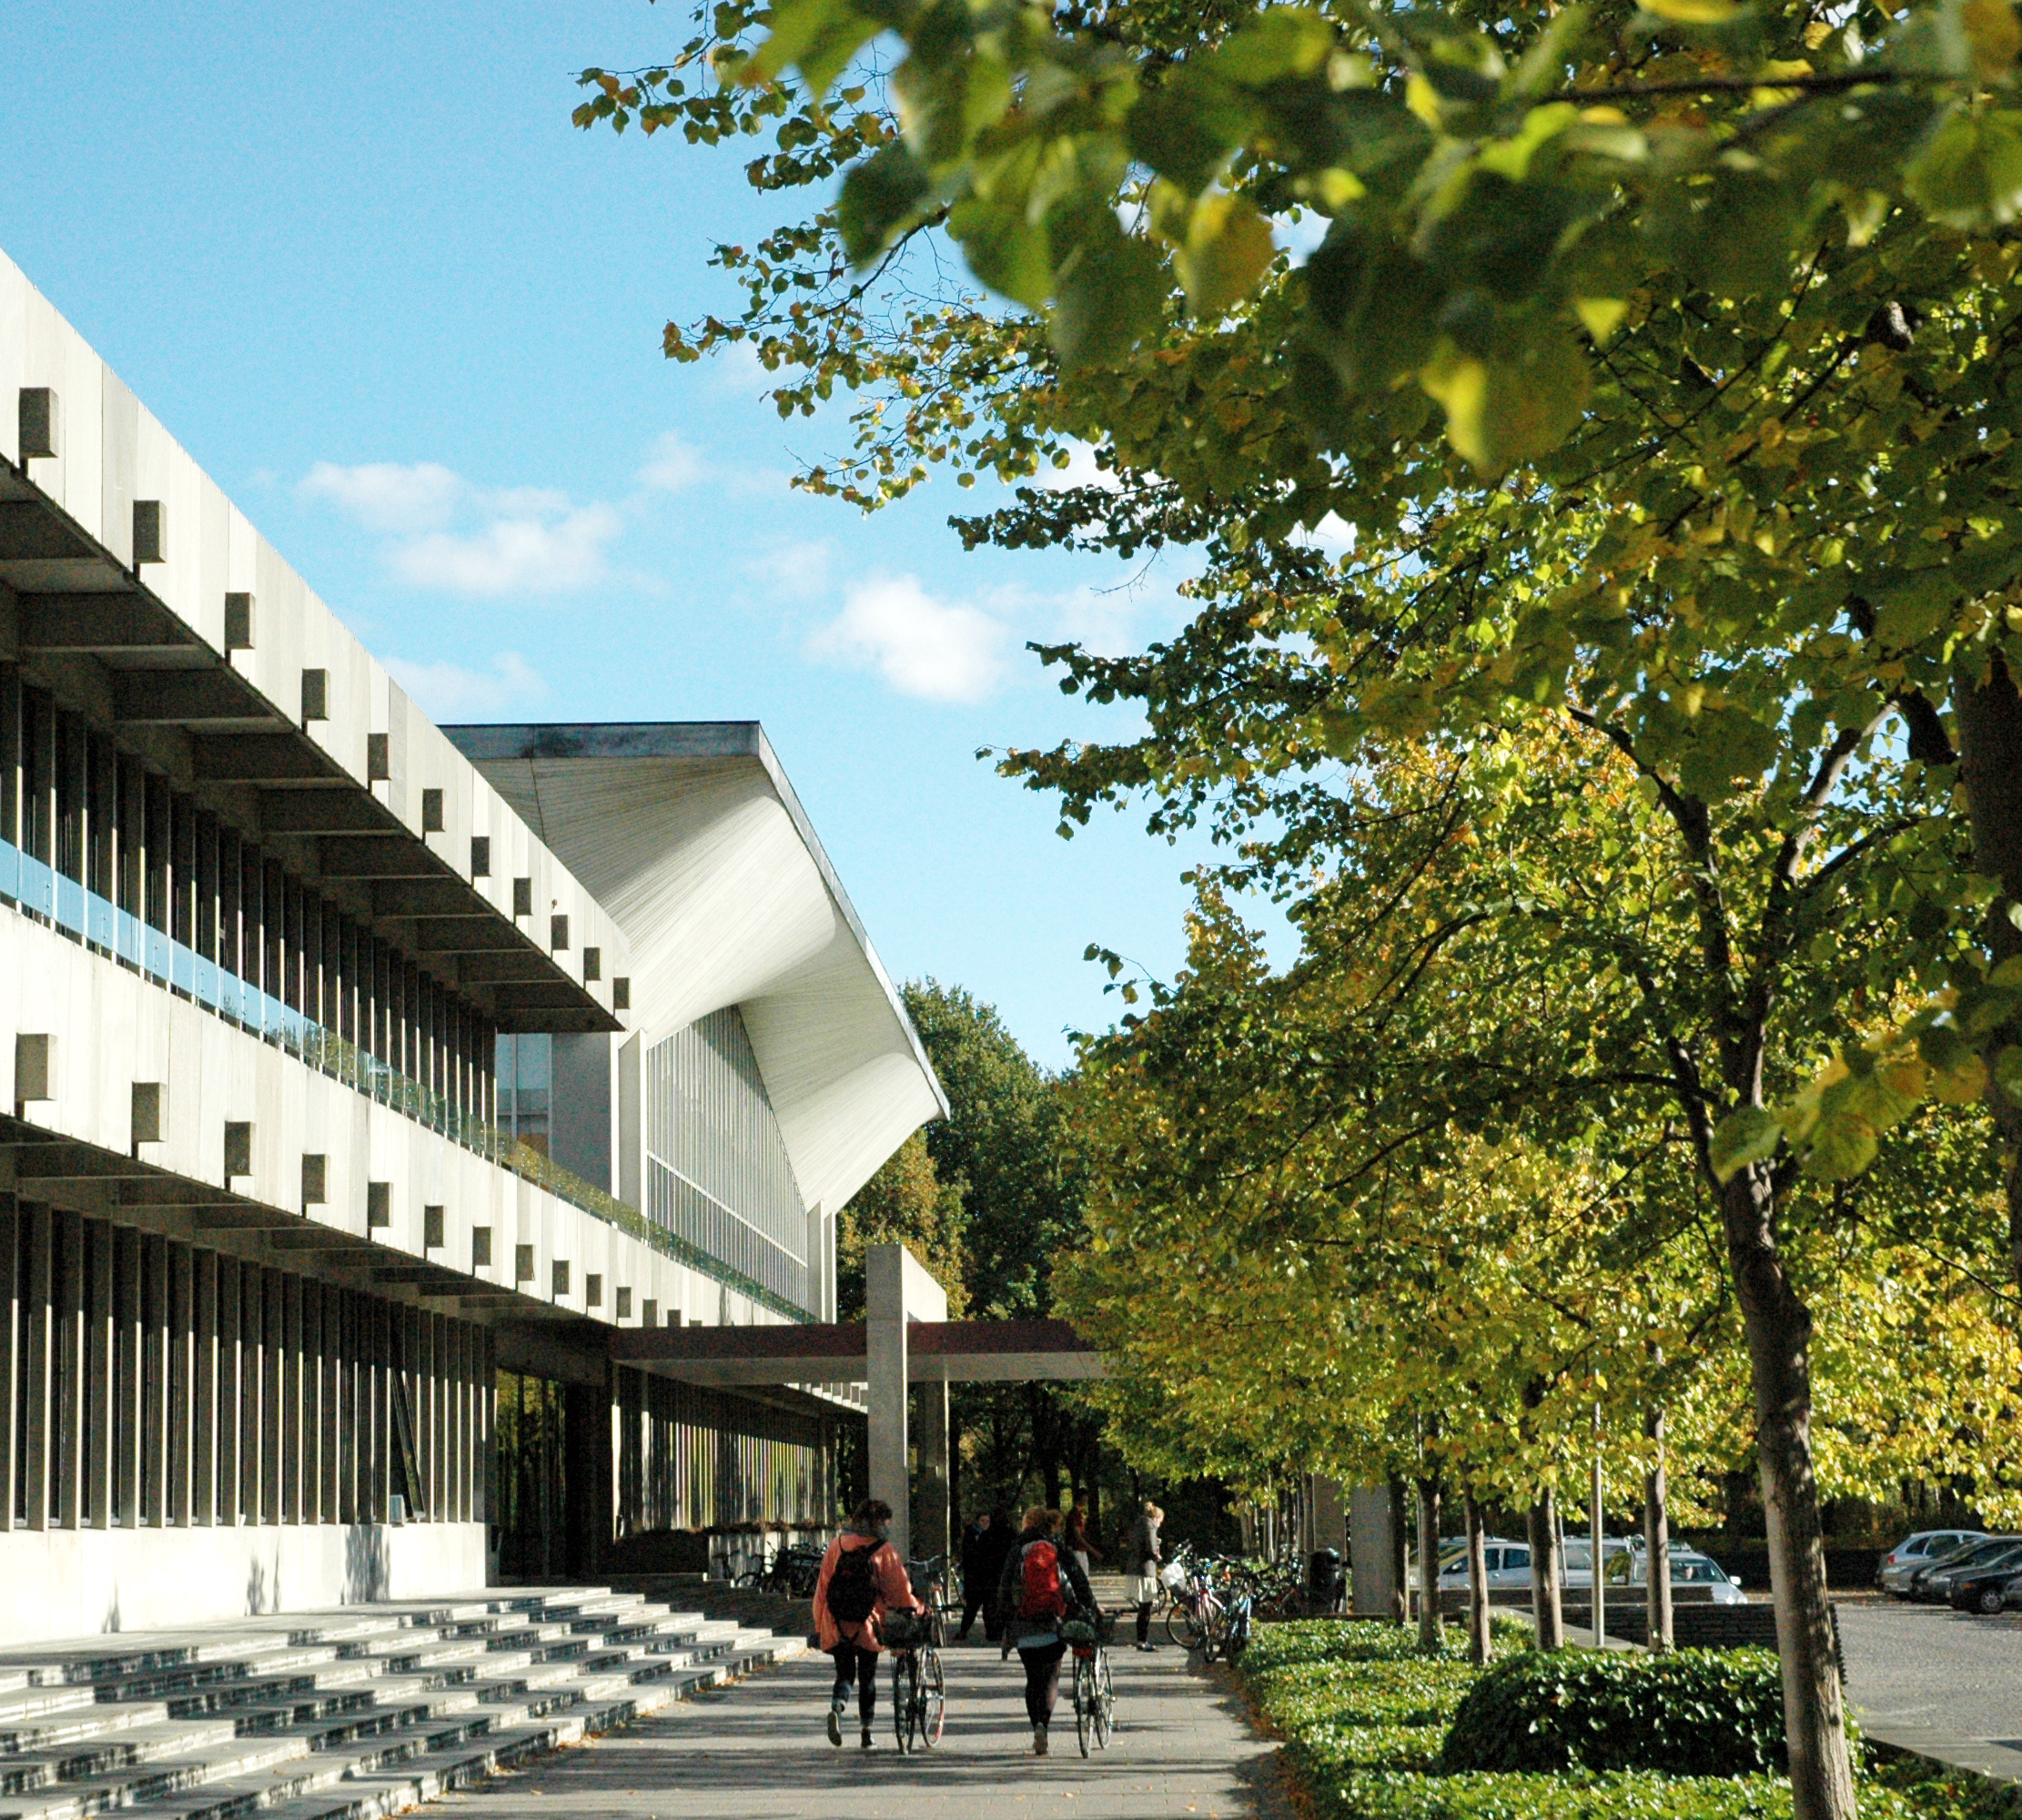
\includegraphics[height=18.9cm,keepaspectratio]{Pictures/DTU_stock_photo.jpg}};
\end{tikzpicture}




\end{titlepage}

\pagecolor{white}
\newgeometry{top=2.81cm, bottom=2.75cm, outer=2.5cm, inner=3.5cm}
\pagestyle{empty}
\cleardoublepage 
\thispagestyle{empty}
\setcounter{page}{1}
\vspace*{\fill}

\textbf{\thesistitle} \newline
\thesissubtitle

\smallskip

\documenttype \newline
\thedate

\smallskip

By \newline
\thesisauthor

\bigskip

\begin{tabularx}{\textwidth}{@{}lX@{}}
    Copyright: & Reproduction of this publication in whole or in part must include the customary bibliographic citation, including author attribution, report title, etc. \\
    Cover photo: & Vibeke Hempler, 2012 \\
    Published by: & DTU, \departmentdescriber, \addressI, \addressII ~Denmark  \\
     & \url{\departmentwebsite} \\
    ISSN: & [0000-0000] (electronic version) \\
    ISBN: & [000-00-0000-000-0] (electronic version) \\
    & \\
    ISSN: & [0000-0000] (printed version) \\
    ISBN: & [000-00-0000-000-0] (printed version)
\end{tabularx}



\clearpage 
\pagestyle{main}
\section*{Approval}
\addcontentsline{toc}{section}{Preface}
This thesis has been prepared over six months at the Section for Indoor Climate, Department of Civil Engineering, at the Technical University of Denmark, DTU, in partial fulfilment for the degree Master of Science in Engineering, MSc Eng. 

It is assumed that the reader has a basic knowledge in the areas of statistics. 

\vfill

\begin{center}
\namesigdate{\thesisauthor~-~\studentnumber}
\end{center}

\vfill


\clearpage 
\section*{Abstract}
\addcontentsline{toc}{section}{Abstract}

\blindtext






\clearpage 
\section*{Acknowledgements}
\addcontentsline{toc}{section}{Acknowledgements}
\textbf{\thesisauthor}, MSc Civil Engineering, DTU \newline
I would like to thank my supervisors for their feedback during my writing of this thesis.

\textbf{Morten Rieger Hannemose}, [Assistant Professor], [affiliation] \newline
[text]

\textbf{[Name]}, [Title], [affiliation] \newline
[text]


\cleardoublepage 
\tableofcontents
\cleardoublepage 

%%%%%%%%%%%%%%%%%%%%%%%%%%%%%%%%%%%%%%%%%%%%%%%%%%%%%%%
\pagenumbering{arabic}
\chapter{Introduction}

In healthcare environments such as hospitals and care homes, data pertaining to critical incidents like falls are scarce due to their infrequent nature and the high privacy requirements surrounding such data. This scarcity poses significant challenges for training robust machine learning models, particularly in applications related to video classification where detailed understanding of such events is crucial. The primary goal of this thesis is to enhance the performance of video classification tasks by leveraging synthetic data, which is designed to closely mirror the underlying distribution of real-world incidents while enabling focused studies on specific, rare events.

To address the challenges inherent in collecting and utilizing real-world data from sensitive environments, this research proposes a novel approach using synthetic data generation. Synthetic data not only adheres to the distributional characteristics of genuine data but also provides flexibility to explore less common scenarios—specifically, those at the tail of the distribution which are typically underrepresented in available datasets.

This work introduces a sophisticated framework for generating synthetic data by explicitly modeling three-dimensional (3D) environments. This includes detailed interactions both among humans and between humans and their surroundings. By integrating these complex interactions as a strong inductive bias, the proposed generative diffusion model enhances the realism and applicability of the synthetic data.

To construct and train this model, we utilize publicly available datasets such as HumanML3D and InterHuman. These datasets include motion capture data of individuals and pairs interacting, each accompanied by textual descriptions. These are combined with 3D scene reconstructions derived from video captures in actual hospital and care home settings. This integration of human motion and scene specifics forms the foundation for our synthetic data generation process.

To effectively reconstruct 3D scenes from the captured videos, we employ state-of-the-art models such as ProHMR and Depth Anything. These models are instrumental in generating per-frame human pose estimations and scene depth labels. These outputs, along with 2D keypoint annotations, are fed into a joint optimization process. This process is critical as it unifies the coordinate systems of the human models and the environment, ensuring that the motion trajectories are smooth and coherent. The result is a highly accurate 3D representation of the scenes, which serves as a vital input for our synthetic data generation.


% This template complies with the DTU Design Guide \url{https://www.designguide.dtu.dk/}. DTU holds all rights to the design programme including all copyrights. It is intended for two-sided printing. The \textbackslash \texttt{cleardoublepage} command can be used to ensure that new sections and the table of contents begins on a right hand page. The back page always ends as an odd page. 

% All document settings have been gathered in Setup/Settings.tex. These are global settings meaning the settings will affect the whole document. Defining the title for example will change the title on the front page, the copyright page and the footer. A watermark can be enabled or disabled in Setup/Premeable.tex. You can edit the watermark to display draft, review, approved, confidential or anything else. By default the watermark is printed on top of the contents of the document and has a transparent grey colour. 

% \section{This is a section}
% Every chapter is numbered and the sections inherit the chapter number followed by a dot and a section number. Figures, equations, tables, ect. also inherit the chapter numbering. 

% \subsection{This is a sub section}
% Sub sections are also numbered. In general try not to use a deep hierarchy of sub sections (\texttt{\textbackslash paragraph\{\}} and the like). The document will become segmented which will make the document appear less coherent. 

% \subsubsection{This is a sub sub section}
% And those are not numbered. It is possible to adjust how deep hierarchy of numbering sections goes in Setup/Settings.tex. 

% The front and back cover have been made to replicate the examples in the design guide \url{https://www.designguide.dtu.dk/#stnd-printmedia}. The name of department heading is omitted  because it is located in the top right corner (no need to write it twice). Take a look at \url{https://www.inside.dtu.dk/en/medarbejder/om-dtu-campus-og-bygninger/kommunikation-og-design/skabeloner/rapporter} if you want to make your cover separately. 

% Citing is done with the \texttt{biblatex} package \cite{biblatex}. Cross referencing (figures, tables, ect.) is taken care by the \texttt{cleveref} package. Just insert the name of the label in \textbackslash \texttt{cref\{\}} and it will automatically format the cross reference. For example writing the \texttt{cleveref} command \textbackslash \texttt{cref\{fig:groupedcolumn\}} will output ``\cref{fig:groupedcolumn}''. Using \textbackslash \texttt{Cref\{\}} will capitalise the first letter and \textbackslash \texttt{crefrange\{\}\{\}} will make a reference range. An example: \Cref{fig:stackedbar} is an example of a stacked bar chart and \crefrange{fig:stackedcolumn}{fig:groupedcolumn} are three consecutive figures.

% \section{Font and symbols test}
% Symbols can be written directly in the document meaning there is no need for special commands to write special characters. I love to write special characters like æøå inside my \TeX{} document. Also á, à, ü, û, ë, ê, î, ï could be nice. So what about the ``¿'' character. What about ° é ® † ¥ ü | œ ‘ @ ö ä ¬ ‹ « © ƒ ß ª … ç ñ µ ‚ · ¡ “ £ ™ [ ] '. Some dashes - – —, and the latex form - -- --- 

% This is a font test \newline 
% Arial Regular \newline 
% \textit{Arial Italic} \newline 
% \textbf{Arial Bold} \newline 
% \textbf{\textit{Arial Bold Italic}}

\cleardoublepage 
\chapter{Background} \label{sec:methods}
\section{Skinned Multi-Person Linear Model (SMPL)}
\begin{figure}[h]
    \centering
    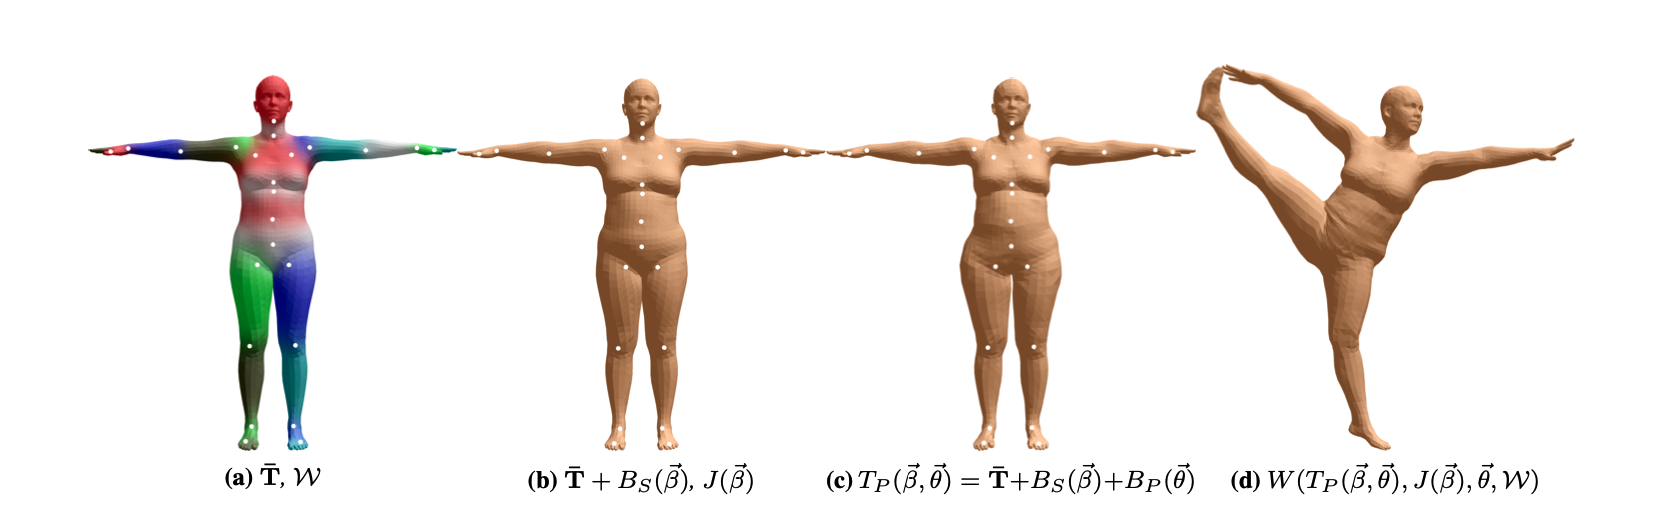
\includegraphics[width=\linewidth]{figures/smpl.png}
    \caption{SMPL model}
\end{figure}
The Skinned Multi-Person Linear (SMPL) model is a parametric body shape model that accurately represents a wide range of human bodies and poses. It is built upon a foundation of linear blend skinning enhanced with corrective blend shapes, which are derived from a large dataset of body scans. The model captures the subtle deformations that occur with different body shapes and poses and can easily be rendered due to its compatibility with existing graphics pipelines. Since its publication, several extensions such as DMPL, incorporating dynamic soft-tissue deformation and SMPL-X, also modelling hands and facial expressions have been introduced. The model is parameterized by $\vec{\beta}$, capturing the variations from a mean body shape and $\vec{\theta}$, specifying the axis-angle rotation of 23 of the template skeleton joints. Mathematically, the model can be expressed as:
\begin{equation}
    M(\vec{\beta}, \vec{\theta}) = W(T_P(\vec{\beta}, \vec{\theta}), J(\vec{\beta}), \vec{\theta}, \mathcal{W})
\end{equation}
where $T_P(\vec{\beta}, \vec{\theta})$ returns the vertices of the rest pose, incorporating the deformations from the body shape and pose and is given by:
\begin{equation}
    T_P(\vec{\beta}, \vec{\theta}) = \vect{\bar{T}} + B_S(\vec{\beta}) + B_P(\vec{\theta})
\end{equation}
$J(\vec{\beta})$ returns the 3D joint locations from the shaped template vertices using a learned regression matrix $\mathcal{J}$ and is given by:
\begin{equation}
    J(\vec{\beta}) = \mathcal{J}(\vect{\bar{T}} + B_S(\vec{\beta}))
\end{equation}
$W$ is the skinning function (e.g. Linear Blend Skinning (LBS) or Dual-Quaternion Blend Skinning (DQBS)) and $\mathcal{W}$ is the blend weights. 

\section{Human Mesh Reconstruction (HMR)}
Recovering the mesh of humans have several applications\dots

\section{Denoising Diffusion Probabilistic Models (DDPM)}
\begin{figure}[H]
    \centering
    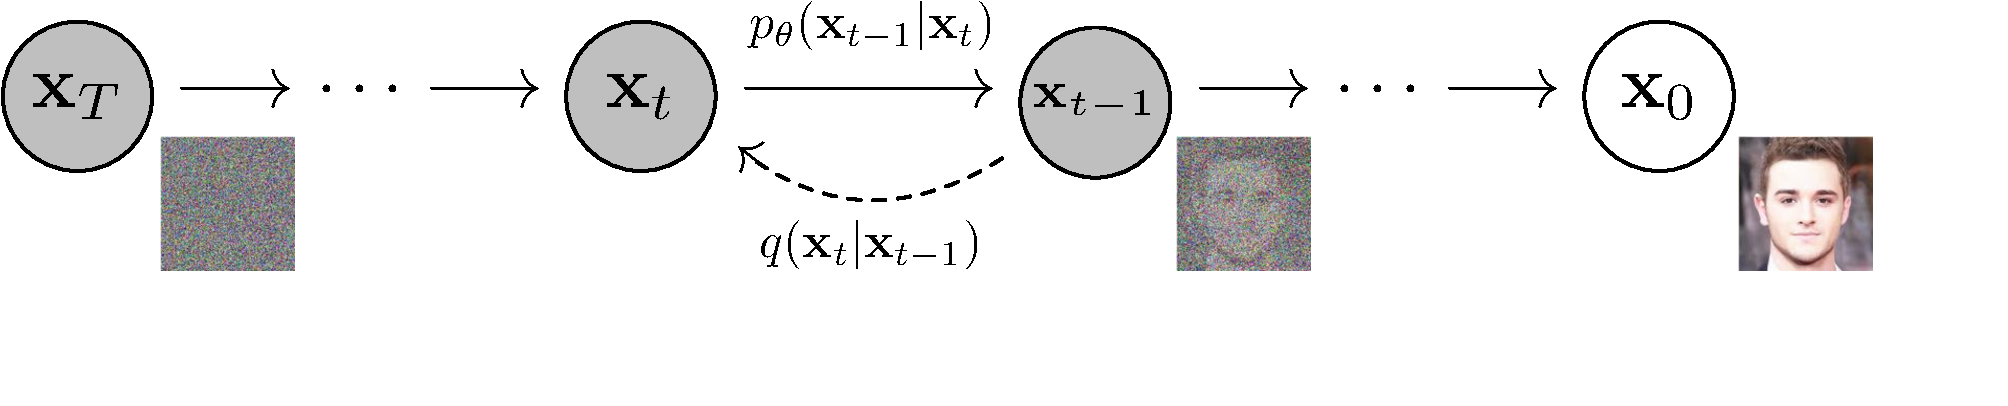
\includegraphics[width=\linewidth]{figures/pgm_diagram_xarrow_small.pdf}
    \caption{Diffusion forward and backward process (taken from \cite{ho2020denoising})}
    \label{fig:diffusion-process}
\end{figure}
In recent years, several types of generative models such as Variational Autoencoders (VAEs), Generative Adverserial Networks (GANs), autoregressive models and flow-based models have shown remarkable results in data generation of varying data modalities, such as images, audio, videos and text. Most recently, Denoising Diffusion Probabilistic Models (DDPMs) have gained large popularity especially within the field of image generation due to several reasons such as high-quality data generation, versitility in several data domains as well as controllability, allowing one to steer the generation towards desired outputs.

A DDPM is a parametarized Markov chain trained using variational inference to reverse a (forward) diffusion process, $q(\vect{x}_{1:T} \mid \vect{x}_0)$, as seen in \cref{fig:diffusion-process} wherein the signal of the data, $\vect{x}_0$, is gradually destroyed by adding gaussian noise according to predefined noise schedule $\{\beta_t  \in (0,1) \}_{t=1}^T$ giving rise to increasingly noisy samples, $\vect{x}_1 \ldots \vect{x}_T$. 

The forward process is defined as follows:
\begin{equation}    
    q(\vect{x}_{1:T} \mid \vect{x}_{0}) = \prod_{t=1}^T q(\vect{x}_{t} \mid \vect{x}_{t-1}), \quad q(\vect{x}_{t} \mid \vect{x}_{t-1}) = \mathcal{N}(x_{t}; \sqrt{1 - \beta_t}\vect{x}_t,\beta_t \vect{I} )
\end{equation}
with $T$ being the discritized number of diffusion steps before all original information is completely discarded. The goal of the inverse or backwards process then becomes to iteratively remove the noise, in order to arrivate at the original data. More formally, the process is defined as:
\begin{equation}
    p_\theta(\vect{x}_{0:T}) = p(\vect{x}_T) \prod_{t=1}^T p_\theta(\vect{x}_{t-1} \mid x_{t}), \quad p_\theta(\vect{x}_{t-1} \mid \vect{x}_{t}) = \mathcal{N}\left(\vect{x}_{t-1}; \vect{\mu}_\theta(\vect{x}_t, t), \vect{\Sigma}_\theta(\vect{x}_t, t) \right)
\end{equation}
taking starting point in pure noise $p(\vect{x}_T) = \mathcal{N}(\vect{x}_T; \vect{0}, \vect{I})$, incrementally removing the noise through the learned functions, $\vect{\mu}_\theta(\vect{x}_t, t)$ and $\vect{\Sigma}_\theta(\vect{x}_t, t)$ commonly parameterized by a deep neural network.
Using the reparameterization trick, we are able to sample any noisy version of our data, $\vect{x}_t$, at time step $t$ given our original data $\vect{x}_0$. Recall our forward transition probability function, $q(\vect{x}_t \mid \vect{x}_{t-1})$. Letting $\alpha_t = 1 - \beta_t$, $\bar{\alpha}_t = \prod_{i=1}^t \alpha_i$ and using the reparameterization trick the expression can be rewritten as:
\begin{equation}
    \vect{x}_t = \sqrt{\alpha_t} \vect{x}_{t-1} + \sqrt{1 - \alpha_t} \epsilon_{t-1}
\end{equation}
where $\epsilon_{t-1} \sim \mathcal{N}(0,1)$. Expanding the recursive definition then gives:
\begin{align*}
    \vect{x}_t    % & = \sqrt{\alpha_t} \vect{x}_{t-1} + \sqrt{1 - \alpha_t} \vect{\epsilon_{t-1}} \\
                    & = \sqrt{\alpha_t} \left( \sqrt{\alpha_{t-1}} \vect{x}_{t-2} + \sqrt{1 - \alpha_{t-1}} \vect{\epsilon}_{t-2} \right) + \sqrt{1 - \alpha_t} \vect{\epsilon_{t-1}} \\
                    % & = \sqrt{\alpha_t \alpha_{t-1}} \vect{x}_{t-2} + \sqrt{\alpha_t(1 - \alpha_{t-1})} \vect{\epsilon_{t-2}} + \sqrt{1 - \alpha_{t}} \vect{\epsilon_{t-1}} \\
                    & = \sqrt{\alpha_t \alpha_{t-1}} \vect{x}_{t-2} + \sqrt{1 - \alpha_{t}\alpha_{t-1}} \vect{\bar{\epsilon}}_{t-2}
\end{align*}
where $\vect{\bar{\epsilon}}_{t-2}$ merges the two independent Gaussians $\vect{\epsilon}_{t-1}$ and $\vect{\epsilon}_{t-2}$ into a single Gaussian with new variance as the sum of variances $\alpha_t (1 - \alpha_{t-1}) + (1 - \alpha_{t}) = 1 - \alpha_t \alpha_{t-1}$. Recursively applying the definition of $\vect{x}_t$ and merging the gaussian noise terms results in the simplified expression:
\begin{equation} \label{eq:nice}
    \vect{x}_t = \sqrt{\bar{\alpha}_t}\vect{x}_0 + \sqrt{1 - \bar{\alpha}_t} \vect{\epsilon}, \quad \vect{\epsilon} \sim \mathcal{N}(\vect{0}, \vect{I})
\end{equation}
% or by undoing the reparameterization:
% \begin{equation}
%     q(\vect{x}_t \vert \vect{x}_0) = \mathcal{N}(\vect{x}_t; \sqrt{\bar{\alpha}_t} \vect{x}_0, (1 - \bar{\alpha}_t)\vect{I})
% \end{equation}
%This result enables sampling of any noisy version of $\vect{x}_t$ at time $t$ given "clean" data $\vect{x}_0$. 
Conversely, given $\vect{x}_0$, the reverse conditional probability:
\begin{equation*}
    q(\vect{x}_{t-1} \vert \vect{x}_t, \vect{x}_0) = \mathcal{N}\left( \vect{x}_{t-1}; \vect{\tilde{\mu}}_t(\vect{x}_t, \vect{x}_0), \tilde{\beta}_t \vect{I} \right)
\end{equation*}
becomes tractable to compute using Bayes rule (derivation in \cref{appendix:q-posterior-derivation}) with mean and variance given by:
\begin{align} \label{eq:x-t-min-1-from-x-t}
    \vect{\tilde{\mu}}_t(\vect{x}_t, \vect{x}_0) &= \frac{\sqrt{\bar{\alpha}_{t-1}} \beta_t}{1-\bar{\alpha}_t} \vect{x}_0+\frac{\sqrt{\alpha_t}\left(1-\bar{\alpha}_{t-1}\right)}{1-\bar{\alpha}_t} \vect{x}_t \overset{\text{Using \ref{eq:nice}}}{=} \frac{1}{\sqrt{\alpha_t}}\left(\vect{x}_t-\frac{1-\alpha_t}{\sqrt{1-\bar{\alpha}_t}} \vect{\epsilon}_t\right) \\
    \tilde{\beta}_t &= \frac{1-\bar{\alpha}_{t-1}}{1-\bar{\alpha}_t} \beta_t
\end{align}
The model is trained by optimizing the variational lower bound on the log likelihood:
\begin{equation}
    L_{VLB}
        = \mathbb{E}_q\left[ \log \frac{p_\theta(\vect{x}_{0:T})}{q(\vect{x}_{1:T} \vert \vect{x}_0)}\right]
        = \mathbb{E}_q\left[\log p(\vect{x_T}) + \sum_{t \geq 1} \log \frac{p_\theta(\vect{x}_{t-1} \vert \vect{x}_{t})}{q(\vect{x}_t \vert \vect{x}_{t-1})}
        \right]
        \leq \mathbb{E}\left[\log p_\theta(\vect{x}_0)\right]
\end{equation}
which in practice means minimizing the negative variational lower bound. 
\cite{ho2020denoising} rewrites this into a sum of KL-divergences:
\begin{equation}
    L_{VLB} = \mathbb{E}_q \left[ \underbrace{D_{\mathrm{KL}} \left(
            q\left(\vect{x}_T \mid \vect{x}_0\right) \| p\left(\vect{x}_T\right)
            \right)}_{L_T} + \sum_{t=2}^T \underbrace{D_{\mathrm{KL}}\left(q\left(\vect{x}_{t-1} \mid \vect{x}_t, \vect{x}_0\right) \| p_\theta\left(\vect{x}_{t-1} \mid \vect{x}_t\right)\right)}_{L_{t-1}} - \underbrace{\log p_\theta\left(\vect{x}_0 \mid \vect{x}_1\right)}_{L_0} \right]
\end{equation}
where the authors model $L_0$ from seperate discrete decoder. As $L_T$ doesn't depend on our parameters, $\theta$, and is therefore constant, it can be ignored during optimization. The rest of the $L_{t-1}$ terms can be efficiently computed in the closed form, by fixing the variance $\vect{\Sigma}_\theta(\vect{x}_t, t) = \sigma_t^2 \vect{I}$ to only depend on the current timestep (authors propose $\sigma_t^2 = \beta_t$ or $\sigma_t^2 = \tilde{\beta}_t$). $L_{t-1}$ can then be written in closed form (derivation in \cref{appendix:L-closed-form}) as:
\begin{equation}
    L_{t-1} = \mathbb{E}_q \left[ \frac{1}{2\sigma_t^2} \| \vect{\tilde{\mu}}_t(\vect{x}_t, \vect{x}_0) - \vect{\mu}_\theta(\vect{x}_t, t) \|^2 \right] + C_t
\end{equation}
where $C_t$ is a constant depending on the choice of $\sigma_t^2$ and the noise schedule. Using \cref{eq:x-t-min-1-from-x-t} \cite{ho2020denoising} reparameterize the expression in terms of predicting the noise:
\begin{equation}
    L_{t-1} = \mathbb{E}_{\vect{x}_0, \vect{\epsilon}}\left[
        \frac{\beta_t^2}{2 \sigma_t^2 \alpha_t \left( 1 - \bar{\alpha}_t\right)} \left\| 
            \vect{\epsilon}-\vect{\epsilon}_\theta \left(\sqrt{\bar{\alpha}_t} \vect{x}_0+\sqrt{1-\bar{\alpha}_t} \vect{\epsilon}, t\right)
            \right\|^2
    \right]
\end{equation}
as they find it leads to better unconditional sample quality when training on the CIFAR10 dataset. Furthermore, they report the best sample quality when using the "simple" objective, ignoring the weighing:
\begin{equation} \label{eq:ddpm-simple-objective}
    L_\mathrm{simple} = \mathbb{E}_{t \sim \mathcal{U}(1, T),\ \vect{\epsilon}} \left[
        \vect{\epsilon} - \vect{\epsilon}_\theta( \sqrt{\bar{\alpha}} \vect{x}_0 + \sqrt{1 - \bar{\alpha}}\vect{\epsilon}, t)
    \right]
\end{equation}

The final training and sampling scheme, as outlined in \cref{alg:training} and \cref{alg:sampling} can be summarized as follows. The training algorithm optimizes the model to predict and remove noise from data, while the sampling algorithm uses the trained model to iteratively transform random noise into structured data.

\algrenewcommand\algorithmicindent{0.5em}%
\begin{figure}[t]
\begin{minipage}[t]{0.495\textwidth}
\begin{algorithm}[H]
  \caption{Training} \label{alg:training}
  \small
  \begin{algorithmic}[1]
    \Repeat
      \State $\vect{x}_0 \sim q(\vect{x}_0)$
      \State $t \sim \mathrm{Uniform}(\{1, \dotsc, T\})$
      \State $\vect{\epsilon}\sim\mathcal{N}(\vect{0},\vect{I})$
      \State Take gradient descent step on
      \Statex $\qquad \grad_\theta \left\| \vect{\epsilon} - \vect{\epsilon}_\theta(\sqrt{\bar\alpha_t} \vect{x}_0 + \sqrt{1-\bar\alpha_t}\vect{\epsilon}, t) \right\|^2$
    \Until{converged}
  \end{algorithmic}
\end{algorithm}
\end{minipage}
\hfill
\begin{minipage}[t]{0.495\textwidth}
\begin{algorithm}[H]
  \caption{Sampling} \label{alg:sampling}
  \small
  \begin{algorithmic}[1]
    \vspace{.04in}
    \State $\vect{x}_T \sim \mathcal{N}(\vect{0}, \vect{I})$
    \For{$t=T, \dotsc, 1$}
      \State $\vect{z} \sim \mathcal{N}(\vect{0}, \vect{I})$ if $t > 1$, else $\vect{z} = \vect{0}$
      \State $\vect{x}_{t-1} = \frac{1}{\sqrt{\alpha_t}}\left( \vect{x}_t - \frac{1-\alpha_t}{\sqrt{1-\bar\alpha_t}} \vect{\epsilon}_\theta(\vect{x}_t, t) \right) + \sigma_t \vect{z}$
    \EndFor
    \State \textbf{return} $\vect{x}_0$
    \vspace{.04in}
  \end{algorithmic}
\end{algorithm}
\end{minipage}
\vspace{-1em}
\end{figure}

% To summarize, diffusion models are generative models that create data by reversing a diffusion process. They are trained using a simplified version of the variational lower bound on the log-likelihood. Starting from pure noise, the model iteratively removes the predicted noise through a step-by-step denoising process, effectively reconstructing the original data. This approach allows DDPMs to produce high-quality and diverse outputs.

\subsection{Variance schedules}
\begin{figure}[H]
    \centering
    \begin{subfigure}[b]{0.49\linewidth}
        \centering
        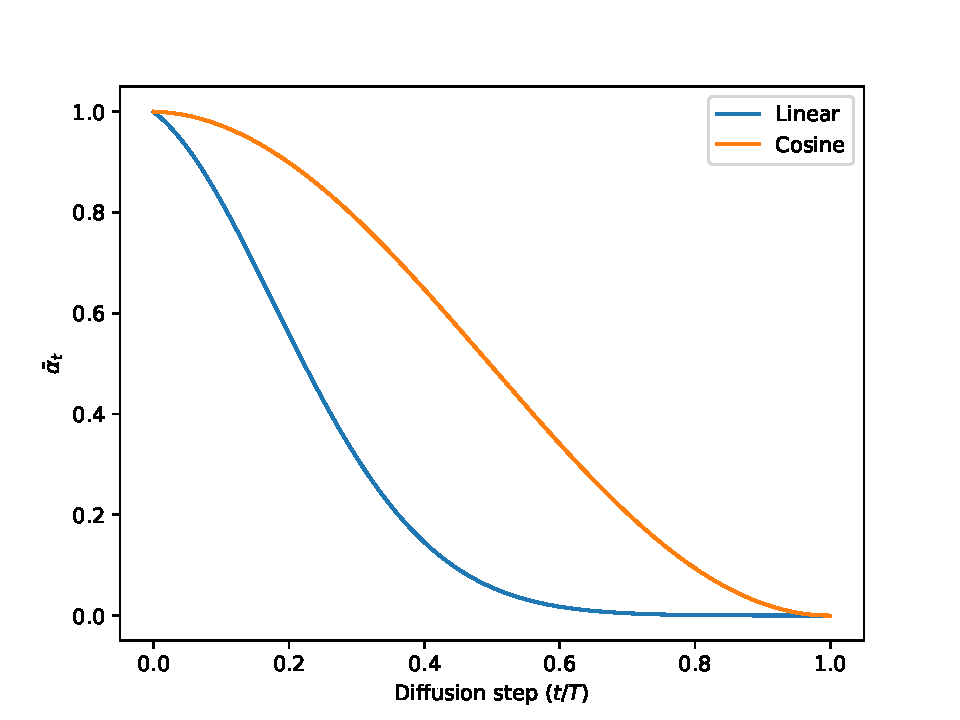
\includegraphics[width=\linewidth]{figures/schedule.pdf}    
    \end{subfigure}
    \hfill
    \begin{subfigure}[b]{0.49\linewidth}
        \centering
        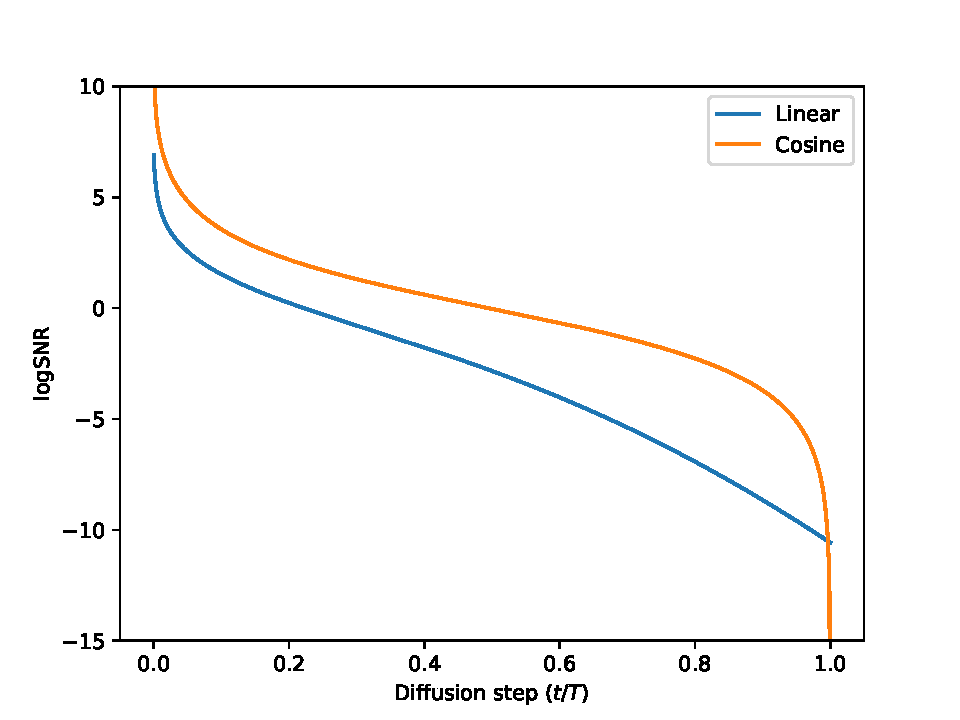
\includegraphics[width=\linewidth]{figures/snr.pdf}    
    \end{subfigure}
    \caption{Linear and cosine schedule and signal-to-noise ratio.}
    \label{fig:schedule}
\end{figure}
In the DDPM paper \cite{ho2020denoising} choose a variance schedule with $\beta_t$ linearly increasing from $\beta_1 = 10^{-4}$ to $\beta_T = 0.02$. However, this results in $\vect{x}_t$ almost entirely losing its signal in the last quarter of the schedule as problematized by \cite{pmlrv139nichol21a}. The authors instead propose a cosine variance schedule, where the squared signal proportion is given by:
\begin{equation}
    \bar{\alpha}_t=\frac{f(t)}{f(0)}, \quad f(t)=\cos \left(\frac{t / T+s}{1+s} \cdot \frac{\pi}{2}\right)^2
\end{equation}
where $s$ controls the offset of the noise schedule. The authors set $s=0.008$ as they found that $s=0$ resulted in minuscule noise near $t=0$ making it hard for the model to predict $\epsilon$. From $\bar{\alpha}_t$ one can then compute $\beta_t = \min\left( 1 - \frac{\bar{\alpha}_t}{\bar{\alpha}_{t-1}}, 0.999 \right)$ with the $\min$ to prevent singularities. A comparison of the cosine and linear schedules can be seen in \cref{fig:schedule}. 


\subsection{Classifier and Classifier-Free Guidance (CFG)}
% When sampling from generative models, one often wants to conditionally generate samples from the data distribution of different sub categories. One method for doing so with diffusion models is classifier guidance. Here the generation process relies on an external model guiding the reverse diffusion process towards the sub category date manifold. We first define the score-function as the gradient of the log-likelihood:
% \begin{equation}
%     s_\theta(\vect{x}) = \grad_{\vect{x}} \log p_\text{data}(\vect{x})
% \end{equation}

% \begin{equation}
%     \dot{\vect{x}} = 
% \end{equation}

% \begin{equation}
%     \grad_{\vect{x}_t} \log p_\theta\left(\vect{x}_t\right)=-\frac{1}{\sqrt{1-\bar{\alpha}_t}} \vect{\epsilon}_\theta\left(\vect{x}_t\right)
% \end{equation}

% \cite{dharial2021diffusion}
In practice, it is often desirable to steer the generation process in order to output data belonging to a specific class, such as cats or dogs in the context of image generation, or incorporating some other information relevant for the output. This process can be framed within the context of probability theory as conditional generation, where the aim is to maximize the probability of the data, $\vect{x}$, given some conditioning signal, $y$, (e.g. a class label. According to Bayes' rule, the conditional probability can be expressed as:
\begin{equation}
    p(\vect{x} \mid y) = \frac{p(\vect{x}, y)}{p(y)} \propto p(y \mid \vect{x}) p(\vect{x})
\end{equation}
Hence, it is proportional to the joint probability of the data and label, which from basic probability theory is equal to the product of the unconditional probability of the data, $p(\vect{x})$, and the probability of the conditioning signal given the data, $p(y \mid \vect{x})$ (for labels; that the data belonging to the given class). In the DDPM paper \cite{ho2020denoising} establishes connection between diffusion models and Noise-Conditioned Score Networks (NCSN) and shows how the reverse diffusion process can be seen as a temporal discritized type of annealed Langevin dynamics given by the stochastic differential equation:
\begin{equation}
    \frac{d}{dt} \log p(\vect{x}_t) = \sqrt{\bar{\alpha}_t} s(\vect{x}_t, t) + \sqrt{1 - \bar{\alpha}_t} \vect{z}_t
\end{equation}
where $z_t \sim \mathcal{N}(0, 1)$ and $s(\vect{x}_t, t) = \grad_{\vect{x}_t} \log p(\vect{x}_t)$ is referred to as the score function. It turns out that the denoising network can be used to approximate the score function:
\begin{equation}
    s(\vect{x}_t, t) \approx -\frac{1}{\sqrt{1 - \bar{\alpha}_t}} \vect{\epsilon}_\theta(\vect{x}_t, t)
\end{equation}
Returning to the factorization of the conditional probability, taking the gradient of the log of both sides reveals the relationship with the score function:
\begin{equation}
    \grad_{\vect{x}_t} \log p(\vect{x}_t \mid y ) = \grad_{\vect{x}_t} \log p(y \mid \vect{x}_t) + \underbrace{\grad_{\vect{x}_t} \log p(\vect{x}_t)}_{s(\vect{x}_t, t)}
\end{equation}
\cite{dharial2021diffusion} trains a classifier, $f_\phi(y \mid \vect{x}_t) \approx p(y \mid \vect{x}_t)$, seperately to predict the class label of noisy images. By using the reformulated denoising function:
\begin{equation}
    \bar{\vect{\epsilon}}_{\theta}(\vect{x}_t, t) = \vect{\epsilon}_\theta(\vect{x}_t, t) - \sqrt{1 - \bar{\alpha}_t} \grad_{\vect{x}_t} \log f_\phi(y \mid \vect{x}_t)
\end{equation}
where $s$ controls guidance strength, it is possible to guide the diffusion sampling e.g. in order to generate images of a specific category, hence the name classifier guidance. 



% Write about classifier-free guidance.
% 



\section{Tranformer architecture}
\begin{figure}[H]
    \centering
    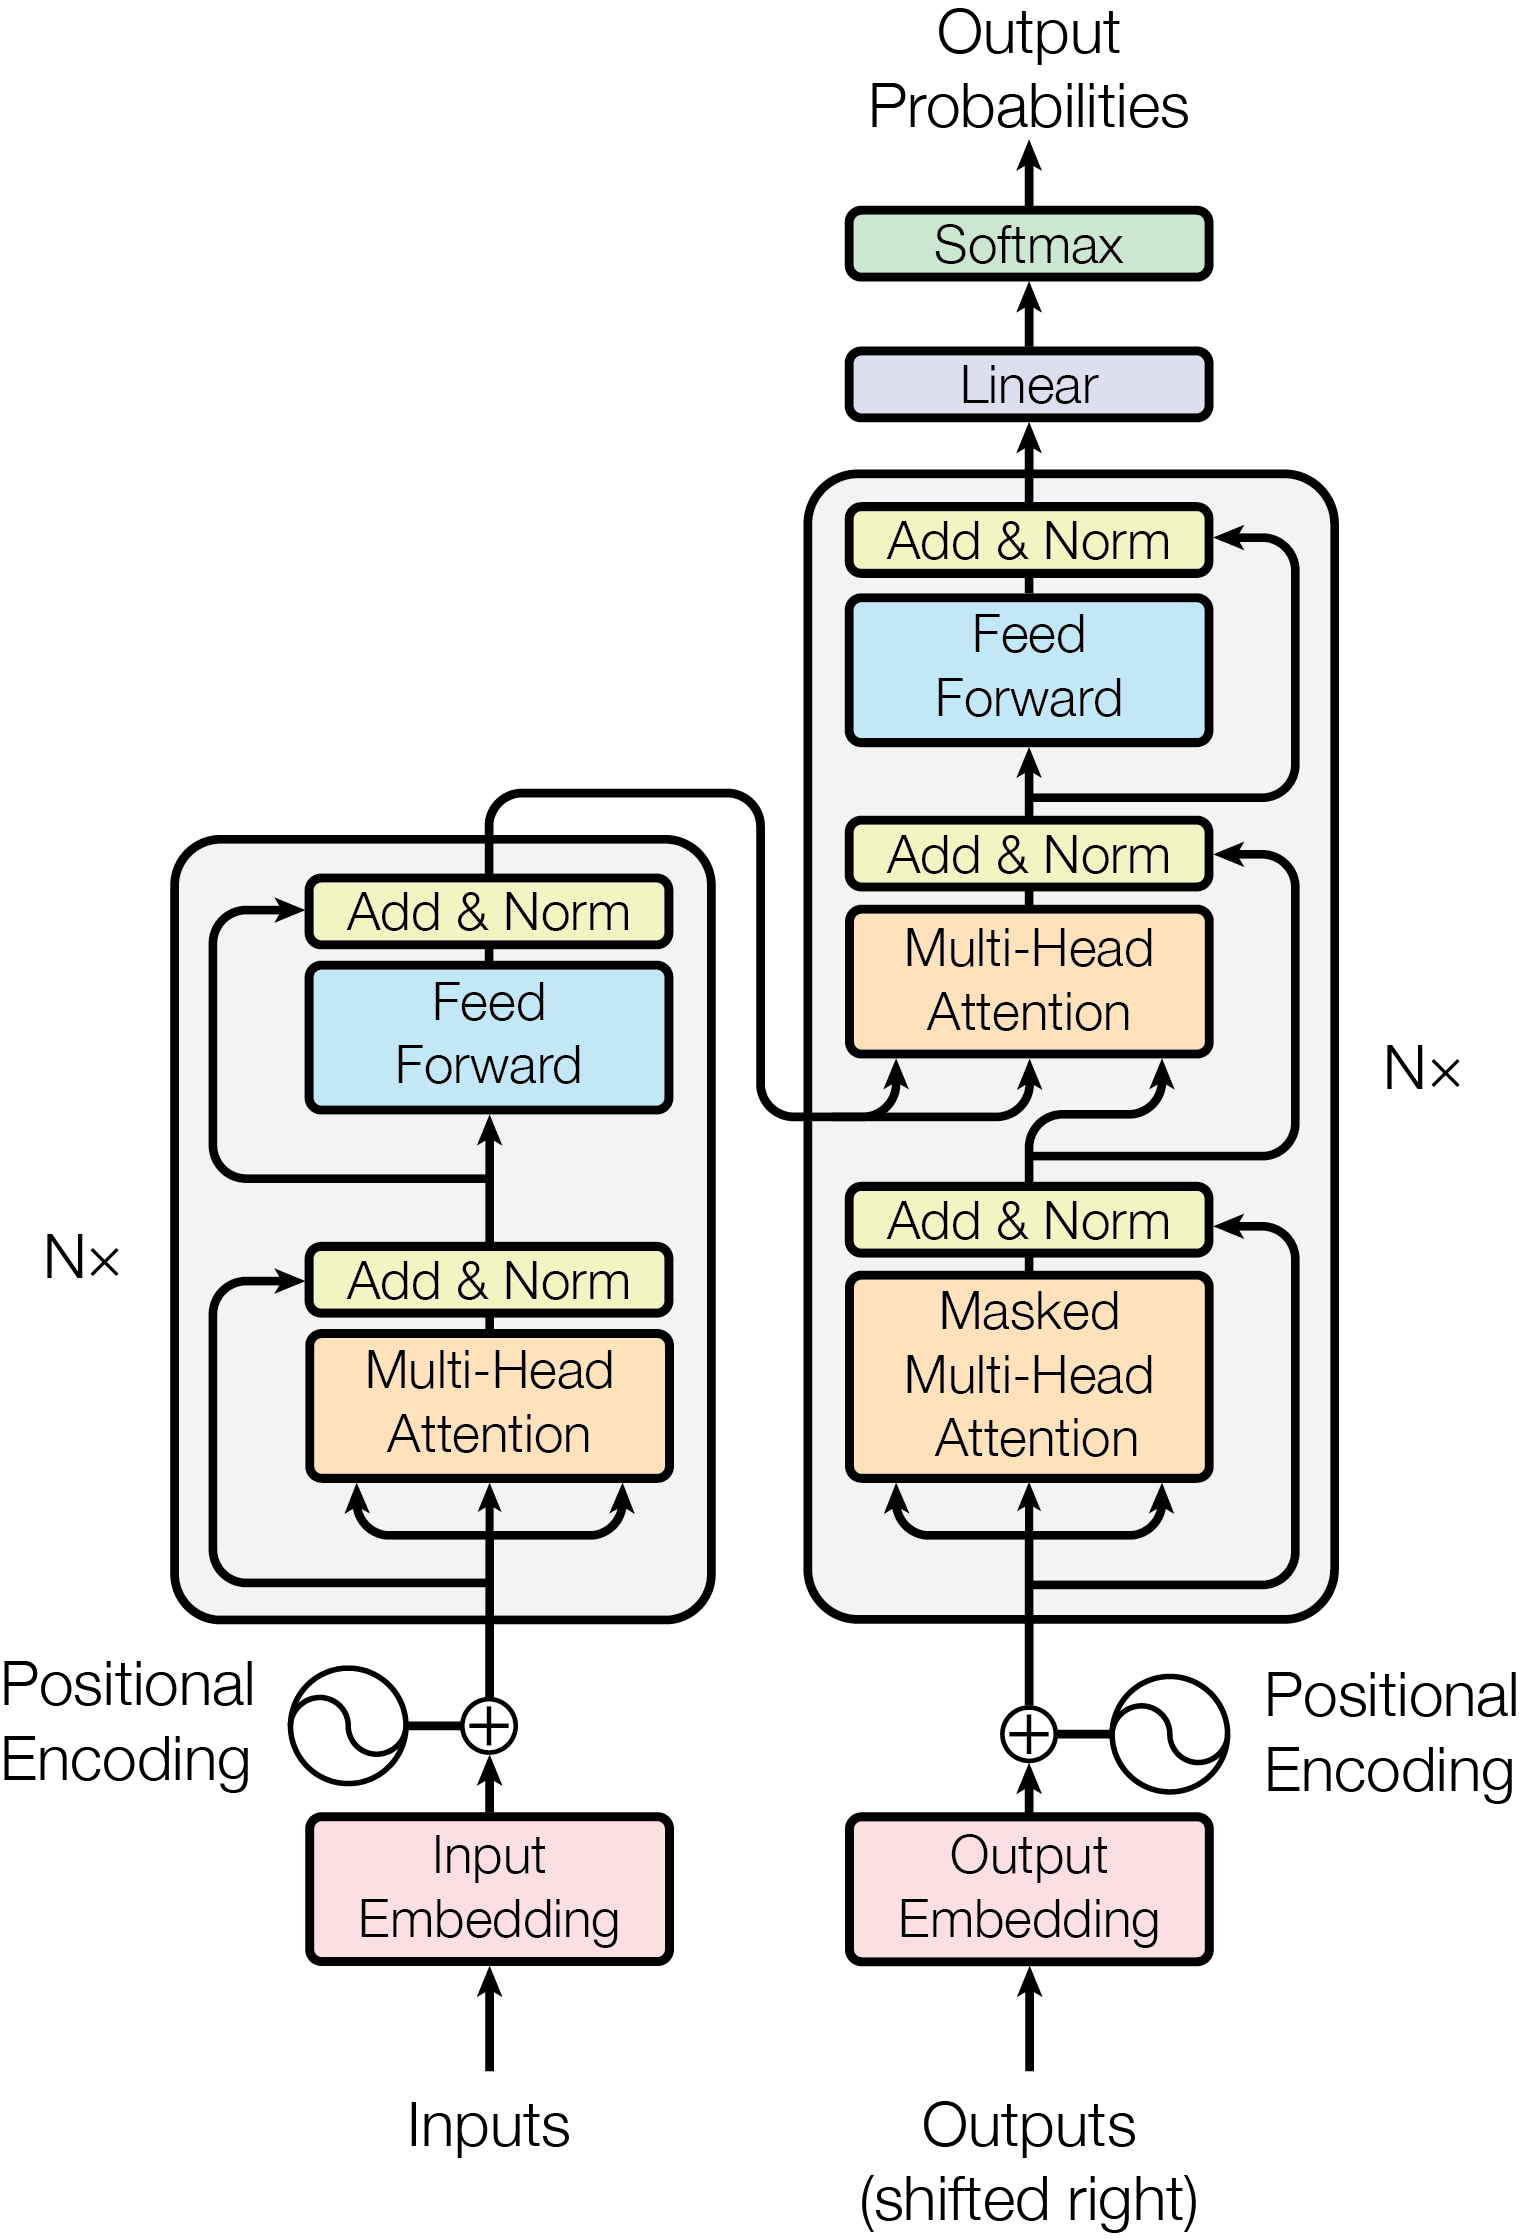
\includegraphics[width=0.4\linewidth]{figures/transformer.png}
    \caption{The transformer (Image from \cite{transformer2017}.)}
\end{figure}
The transformer model, introduced by \cite{transformer2017}, revolutionized natural language processing (NLP) and machine translation. This model was designed as an alternative to the traditional recurrent sequence models, such as the seq2seq model by \cite{seq2seq}, which had been widely used in NLP tasks.
\begin{figure}[H]
    \centering
    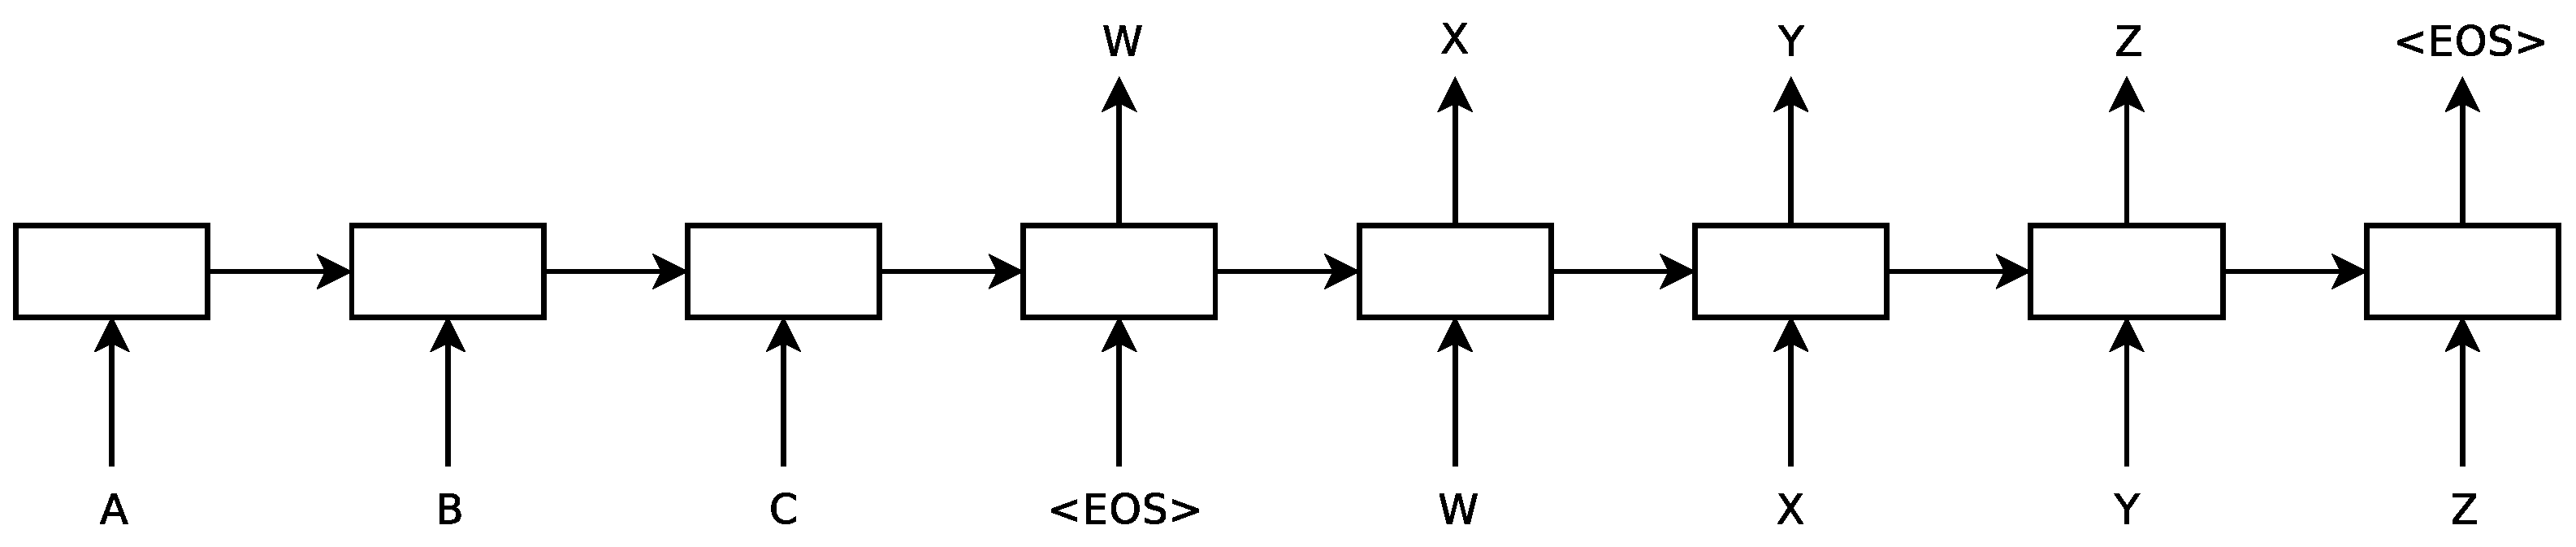
\includegraphics[width=0.8\linewidth]{figures/seq2seq.eps}
    \caption{The seq2seq model by \cite{seq2seq}.}
    \label{fig:seq2seq}
\end{figure}
The seq2seq model (as illustrated in \cref{fig:seq2seq}) encodes an input sequence into a context vector and then decodes the output sequence from this vector in a sequential manner. This approach often results in an information bottleneck, particularly when dealing with long-range dependencies within the data.

In contrast, the transformer model utilizes an attention mechanism, enabling more effective communication between tokens without relying on sequential processing of hidden states. The architecture comprises an encoder and a decoder. The encoder uses multi-headed self-attention to create semantic representations for each token in the input sequence, allowing the model to process the entire context simultaneously.

The decoder then uses these representations through cross-attention and causal self-attention mechanisms. Cross-attention integrates information from the encoder's output, while causal self-attention ensures that the model only considers previously generated tokens, maintaining the autoregressive nature crucial for sequential generation tasks.

One of the key strengths of the transformer model is its training efficiency, owing to the parallelizable nature of the attention mechanism. During the generation process, tokens are produced in an autoregressive fashion, with each generated token serving as context for the subsequent one.

The transformer's attention mechanism is based on scaled dot-product attention, defined by the following equation:

\begin{equation}
    \text{Attention}(Q, K, V) = \text{softmax}\left(\frac{Q K^T}{\sqrt{d_k}} \right) V
\end{equation}
$Q$, $K$ and $V$ are the query, key, and value matrices, respectively, and $d_k$ is the dimension of the key vectors.

For causal self-attention, the model masks future tokens for each key to prevent information leakage, ensuring the model attends only to past and present tokens during both training and inference.

Since the transformer architecture does not inherently encode positional information, Vaswani et al. introduced a sinusoidal positional encoding scheme. This scheme incorporates positional information into each element of the input sequence, defined as:



\section{Human Motion Generation}
Generating realistic human motion has several applications 


- Human Motion Diffusion
- 



\cleardoublepage 
\chapter{Data}
\section{HumanML3D}
The HumanML3D dataset combines the HumanAct12 and AMASS datasets, integrating human motion captured using advanced motion capturing systems and converting the data to a unified parameterization. It covers a broad range of daily human activities, providing 14,616 motions in total, accompanied by 44,970 single-sentence descriptions. Each motion clip includes 3-4 descriptions, and the entire dataset amounts to 28.59 hours of recorded motion. Additionally, the data is augmented by mirroring all motions, with corresponding adjustments to descriptions, such as changing “clockwise” to “counterclockwise.”


\section{InterHuman}
The InterHuman dataset is a comprehensive, large-scale 3D dataset designed to capture human interactive motions involving two individuals. It includes approximately 107 million frames detailing a wide range of human interactions, from professional activities to daily social behaviors. Each motion sequence is paired with natural language annotations, totaling 23,337 descriptions, which provide context and detail for the captured interactions, enhancing the dataset’s utility for training and evaluating models.

\section{Teton dataset}
10s of video with 10 frames per second.
Pseudo dataset of SMPL pose predictions from HMR2.0 for each frame

% The dataset is structured by different levels. Top level is the department, next level is device/particular room, then date and time follows.

\cleardoublepage 
\chapter{Methods}

\section{Tracking \& Matching}
We track the predicted staff and patients across multiple frames, indicated by $t = 1 \ldots T$, by iteratively assigning the predictions, $\{ P_i^{(t)} \}_{i=1}^{M_t}$, to the latest known tracks, $\{ Q^{(t)}_{j} \}_{j=1}^{N_t}$ by greedily picking the assignment with the minimum cost:
\begin{equation}
    \argmin_{i,j} \mathcal{L}_\text{track}(P^{(t)}_i, Q^{(t-1)}_j),
\end{equation}
until either all predictions or latest tracks have been assigned exactly once. In the case of any unassigned predictions, a new track is initialized. After tracks have been assigned, the latest track $Q^{(t)}_j$ is updated with the assigned predictions. We choose the following composite loss function:
\begin{equation}
    \mathcal{L}_\text{track}(P, Q) = \alpha \norm{P_\text{3D kpts} - Q_\text{3D kpts}}{2} + \beta \norm{P_\text{class} - Q_\text{class}}{\infty},
\end{equation}
incorporating both the Euclidean distance between the 3D joint keypoints as well as the predicted person class (staff/patient), with $\alpha$ and $\beta$ weighting the influence of each term. The tracks, $T_i$, are then greedily matched to the ground truth annotations $G_j$, minimizing the loss:
\begin{equation}
    \mathcal{L}_\text{match}(T, G) = \sum_t^{T} \begin{cases}
        \norm{a^{(t)}_{\text{track}, \text{2D kpts}} - b^{(t)}_{\text{track}, \text{2D kpts}}}{2} & \text{if}\ a^{(t)}_\text{track} \in a_\text{track} \\
        \gamma & \text{otherwise}
    \end{cases}
\end{equation}
over the trajectory time horizon $t = 1,2,\ldots,T$ where $\gamma$ is the punishment for not detecting the person.

\section{Human pose sequence optimization}
% Something about using the original poses + vPoser (human pose prior) + annotated keypoints.

\section{3D scene reconstruction}


% Two approaches 

% First approach:
% First uses the relative depth disparity maps and the rendered SMPL poses in order to restore the 
% metric depth scale and offset.
% Pros:
% - Relative depth maps are often more accurate and easier for a model to learn.
% Cons:
% - The process of restoring scale and offset is not very robust and can be prone to errors if the SMPL poses don't overlap precisely with the predicted depths.  
% - The reliance of poses at different distances in order to optimally regress the scale and offset parameters.

% Second approach:
% Using metric depth estimation
% Pros:
% - Doesn't rely on rendering SMPL poses and restoring scale and offset.
% - Domain is contained to indoor hospital and carehome rooms.
% Cons:
% - Less accurate predictions


\subsection*{Restoring depth scale and offsets}
We utilize pseudo ground truth disparity maps generated by the Depth Anything model, inversely proportional to the scene depth, in order to reconstruct a point cloud of the scene. To recover the depth scale and offset we rasterize the predicted SMPL poses, extract the z-buffer, compute the inverse depth and regress the intersection with the normalized disparity maps using the Random Sample Consensus (RANSAC) algorithm robust to outliers. 

\begin{equation}
    \begin{bmatrix}p
        x \\ y \\ 1/z \\ 1
    \end{bmatrix} = \begin{bmatrix}
        f_x & 0 & 0 & p_x \\
        0 & f_y & 0 & p_y \\
        0 & 0 & 1 & 0 \\
        0 & 0 & 0 & 1
    \end{bmatrix} \begin{bmatrix}
        X \\ Y \\ Z \\ 1
    \end{bmatrix}
\end{equation}


\begin{equation}
    X = \frac{Z}{f_x} \left( x - p_x \right) , \quad Y = \frac{Z}{f_x} \left(y - p_y \right)
\end{equation}
where $f_x$, $f_y$ are the horizontal and vertical focal lenghts respectively and ($p_x$, $p_y$) is the principal point often chosen as the center $(w/2,h/2)$ of the image. 

\section{Aligning datasets}
\begin{figure}
    \centering
    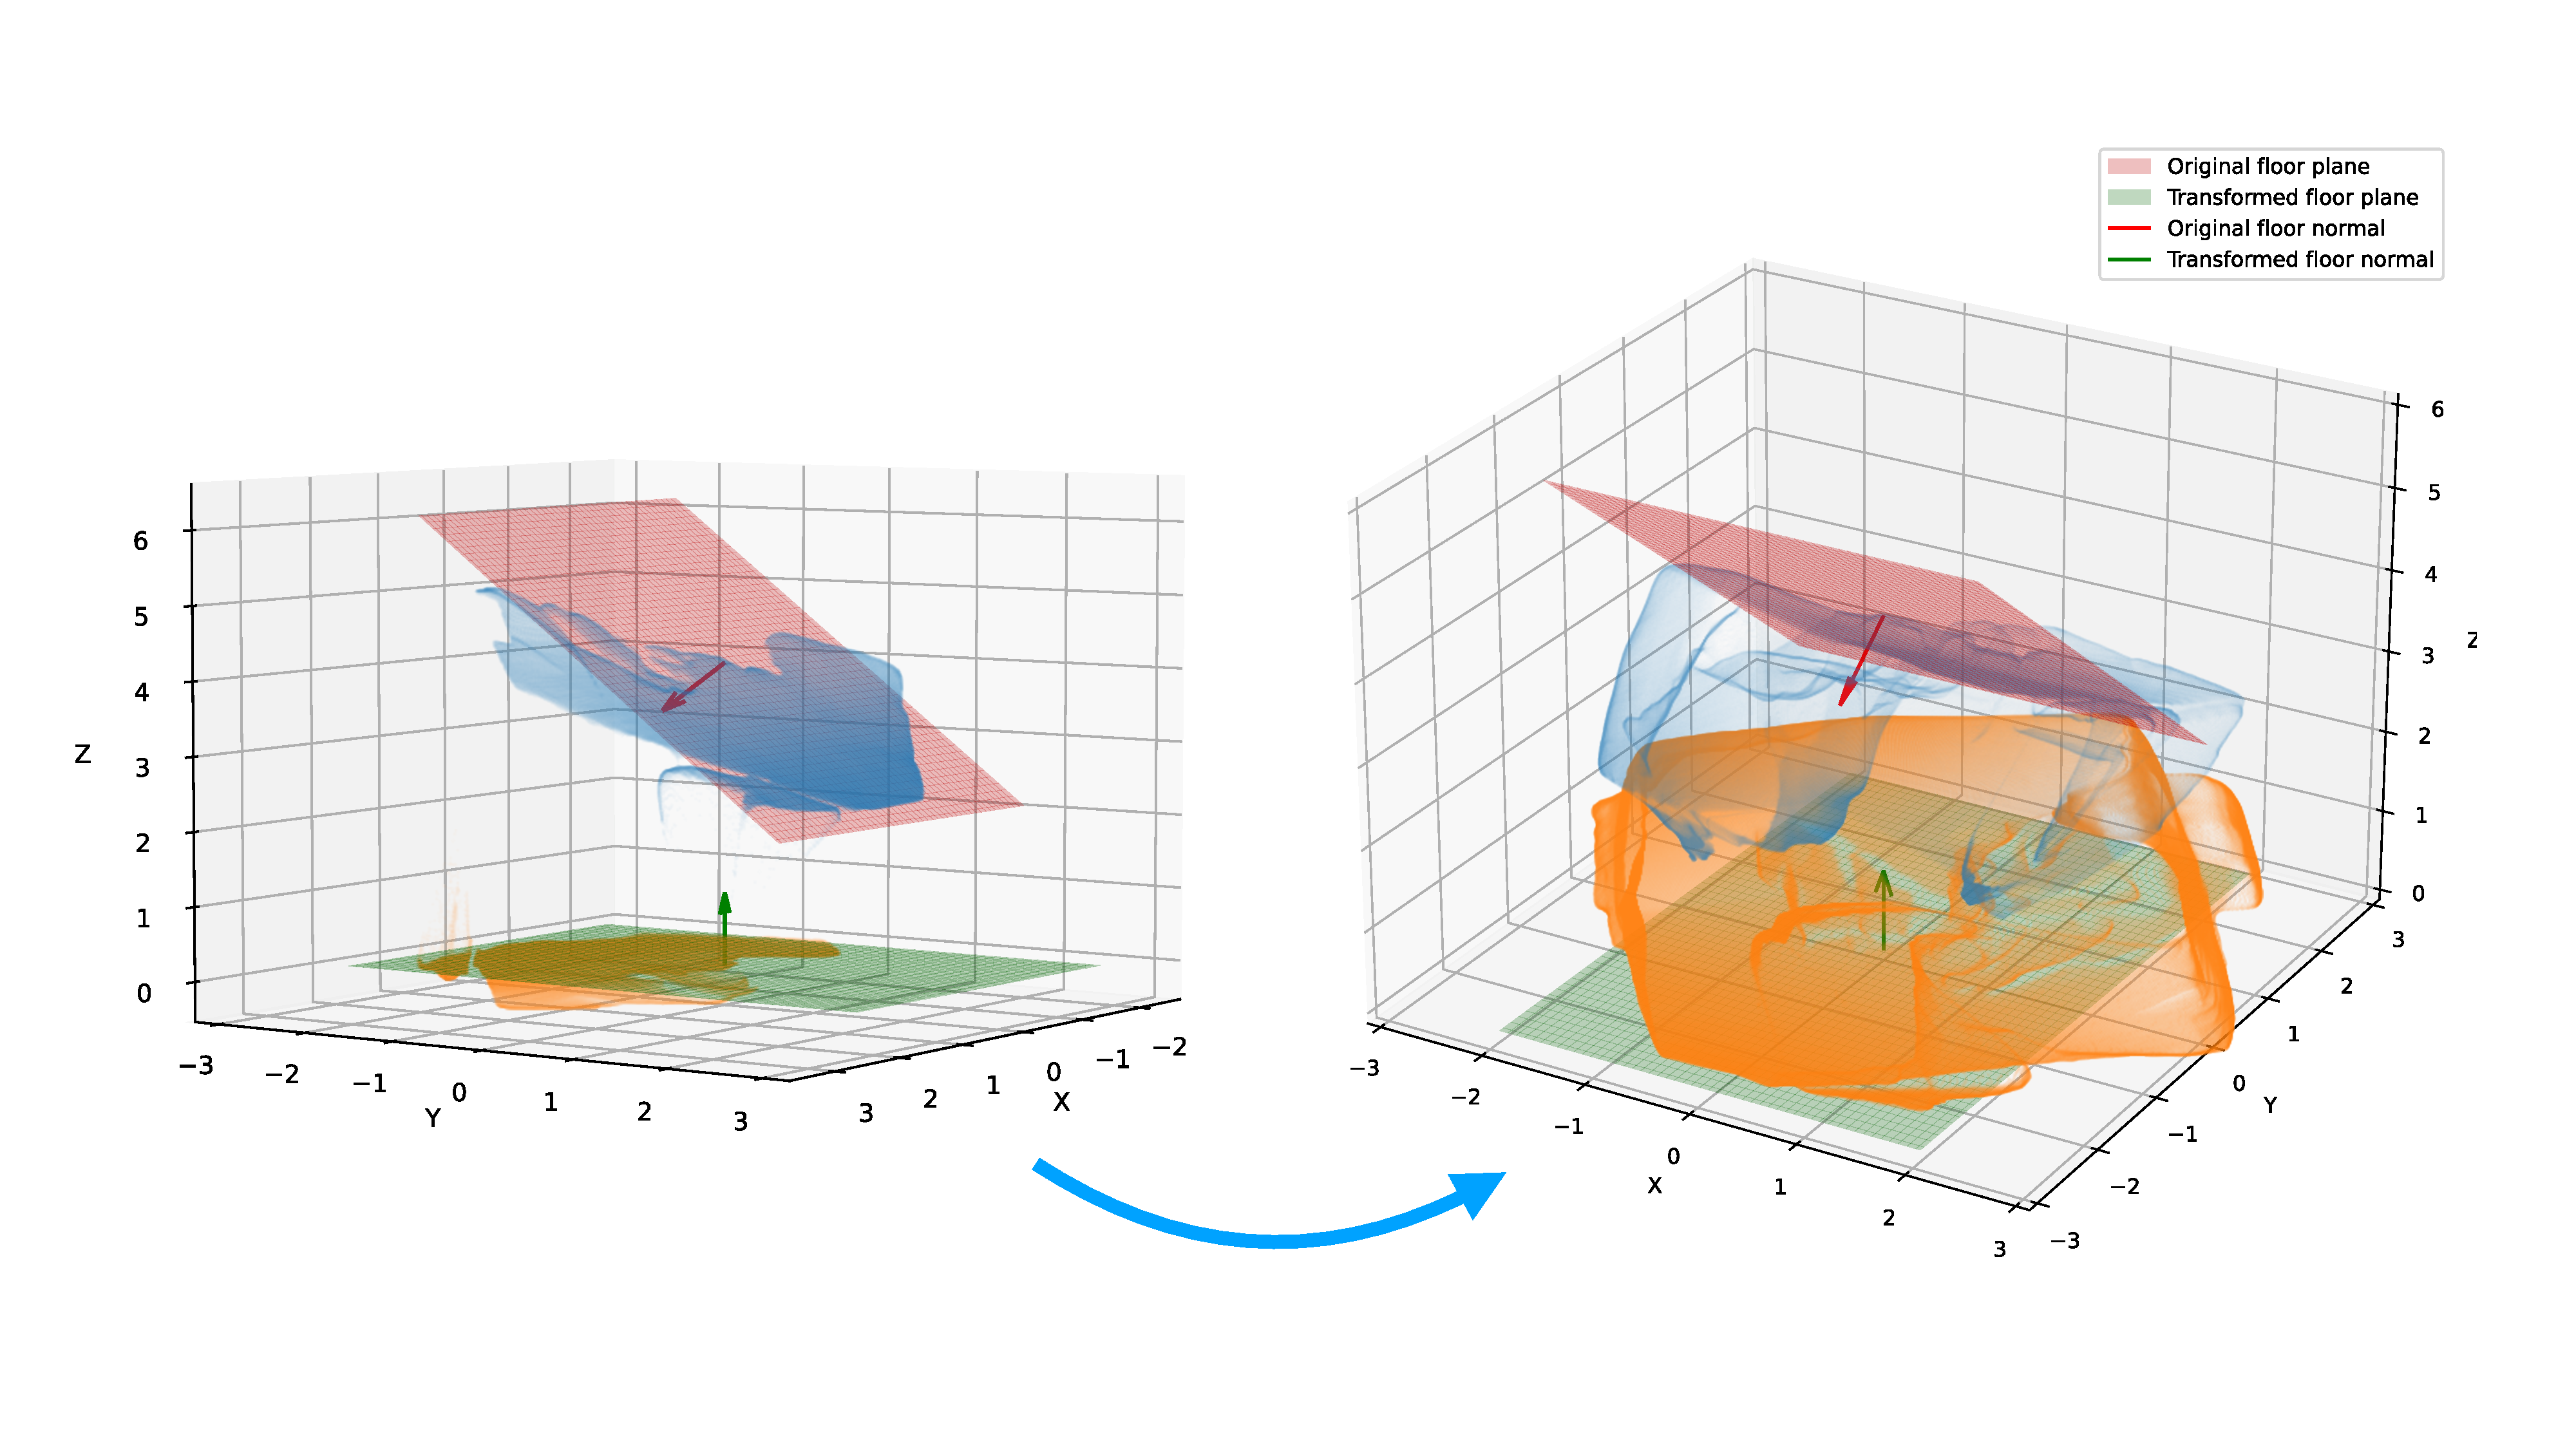
\includegraphics[width=\linewidth]{figures/rotation.pdf}
    \caption{Translation and rotation of room point cloud to align floor with XY-plane.}
    \label{fig:rotate-floor-planes}
\end{figure}

To compute the rotation matrix that aligns the normal vector $\hat{\vect{n}}_\text{floor} = \vect{n}_\text{floor} / \| \vect{n}_\text{floor} \|$ (where $\vect{n}_\text{floor} = (0, 1, \vect{b}_1)^T \times (1, 0, \vect{b}_0)^T$) of the floor plan in the camera coordinate system with the normal vector $\vect{n}_{xy} = (0, 0, 1)$ of the xy-plane, we can utilize Rodrigues' rotation formula. 

First, we construct the skew-symmetric matrix $\mathbf{K}$ from the components of the cross product vector $\vect{v} = \hat{\vect{n}}_\text{floor} \times \vect{n}_{xy}$. The skew-symmetric matrix $\mathbf{K}$ is defined as:
\begin{equation}
    \mathbf{K} = \begin{bmatrix}
        0 & -v_3 & v_2 \\
        v_3 & 0 & -v_1 \\
        -v_2 & v_1 & 0
    \end{bmatrix}
\end{equation}

Next, we compute the rotation matrix $\mathbf{R}$ using Rodrigues' rotation formula. The formula incorporates the identity matrix $\mathbf{I}$, the skew-symmetric matrix $\mathbf{K}$, and a scaling term based on the angle between the vectors. The resulting rotation matrix is given by:

\begin{equation}
    \mathbf{R} = \mathbf{I} + \mathbf{K} + \mathbf{K}^2 \left(\frac{1 - c}{s^2}\right)
\end{equation}

Here, $\mathbf{I}$ is the identity matrix, $c$ is the dot product of $\mathbf{a}$ and $\mathbf{b}$, and $s$ is the norm of the cross product vector $\mathbf{v}$. This formula ensures that the rotation matrix $\mathbf{R}$ not only aligns $\mathbf{a}$ with $\mathbf{b}$ but also preserves the orthogonality and orientation of the coordinate system.

Finally, we transform the point cloud by translating it to align the floor plane intercept with the origin, followed by rotating it using the computed rotation matrix:

\begin{equation}
    \vect{p}^* = \mathbf{R} \left(\vect{p} - (0, 0, b_0)^T \right) 
\end{equation}




\section{Motion and scene representation}
Previous work on single human motion generation uses a canonical representation 

We use a 6D continuous representation of the joint angles as according to \cite{Zhou_2019_CVPR}.
% We represent the motion similar to 


\section{Diffusion model}




\cleardoublepage 
\chapter{Results}
\section*{Motion Estimation}
\begin{figure}
    \centering
    \includegraphics[width=\linewidth]{figures/results/motion1.png}
    \caption{Example of bad annotations effect on estimated motion.}
    \label{fig:motion1}
\end{figure}

\begin{figure}
    \centering
    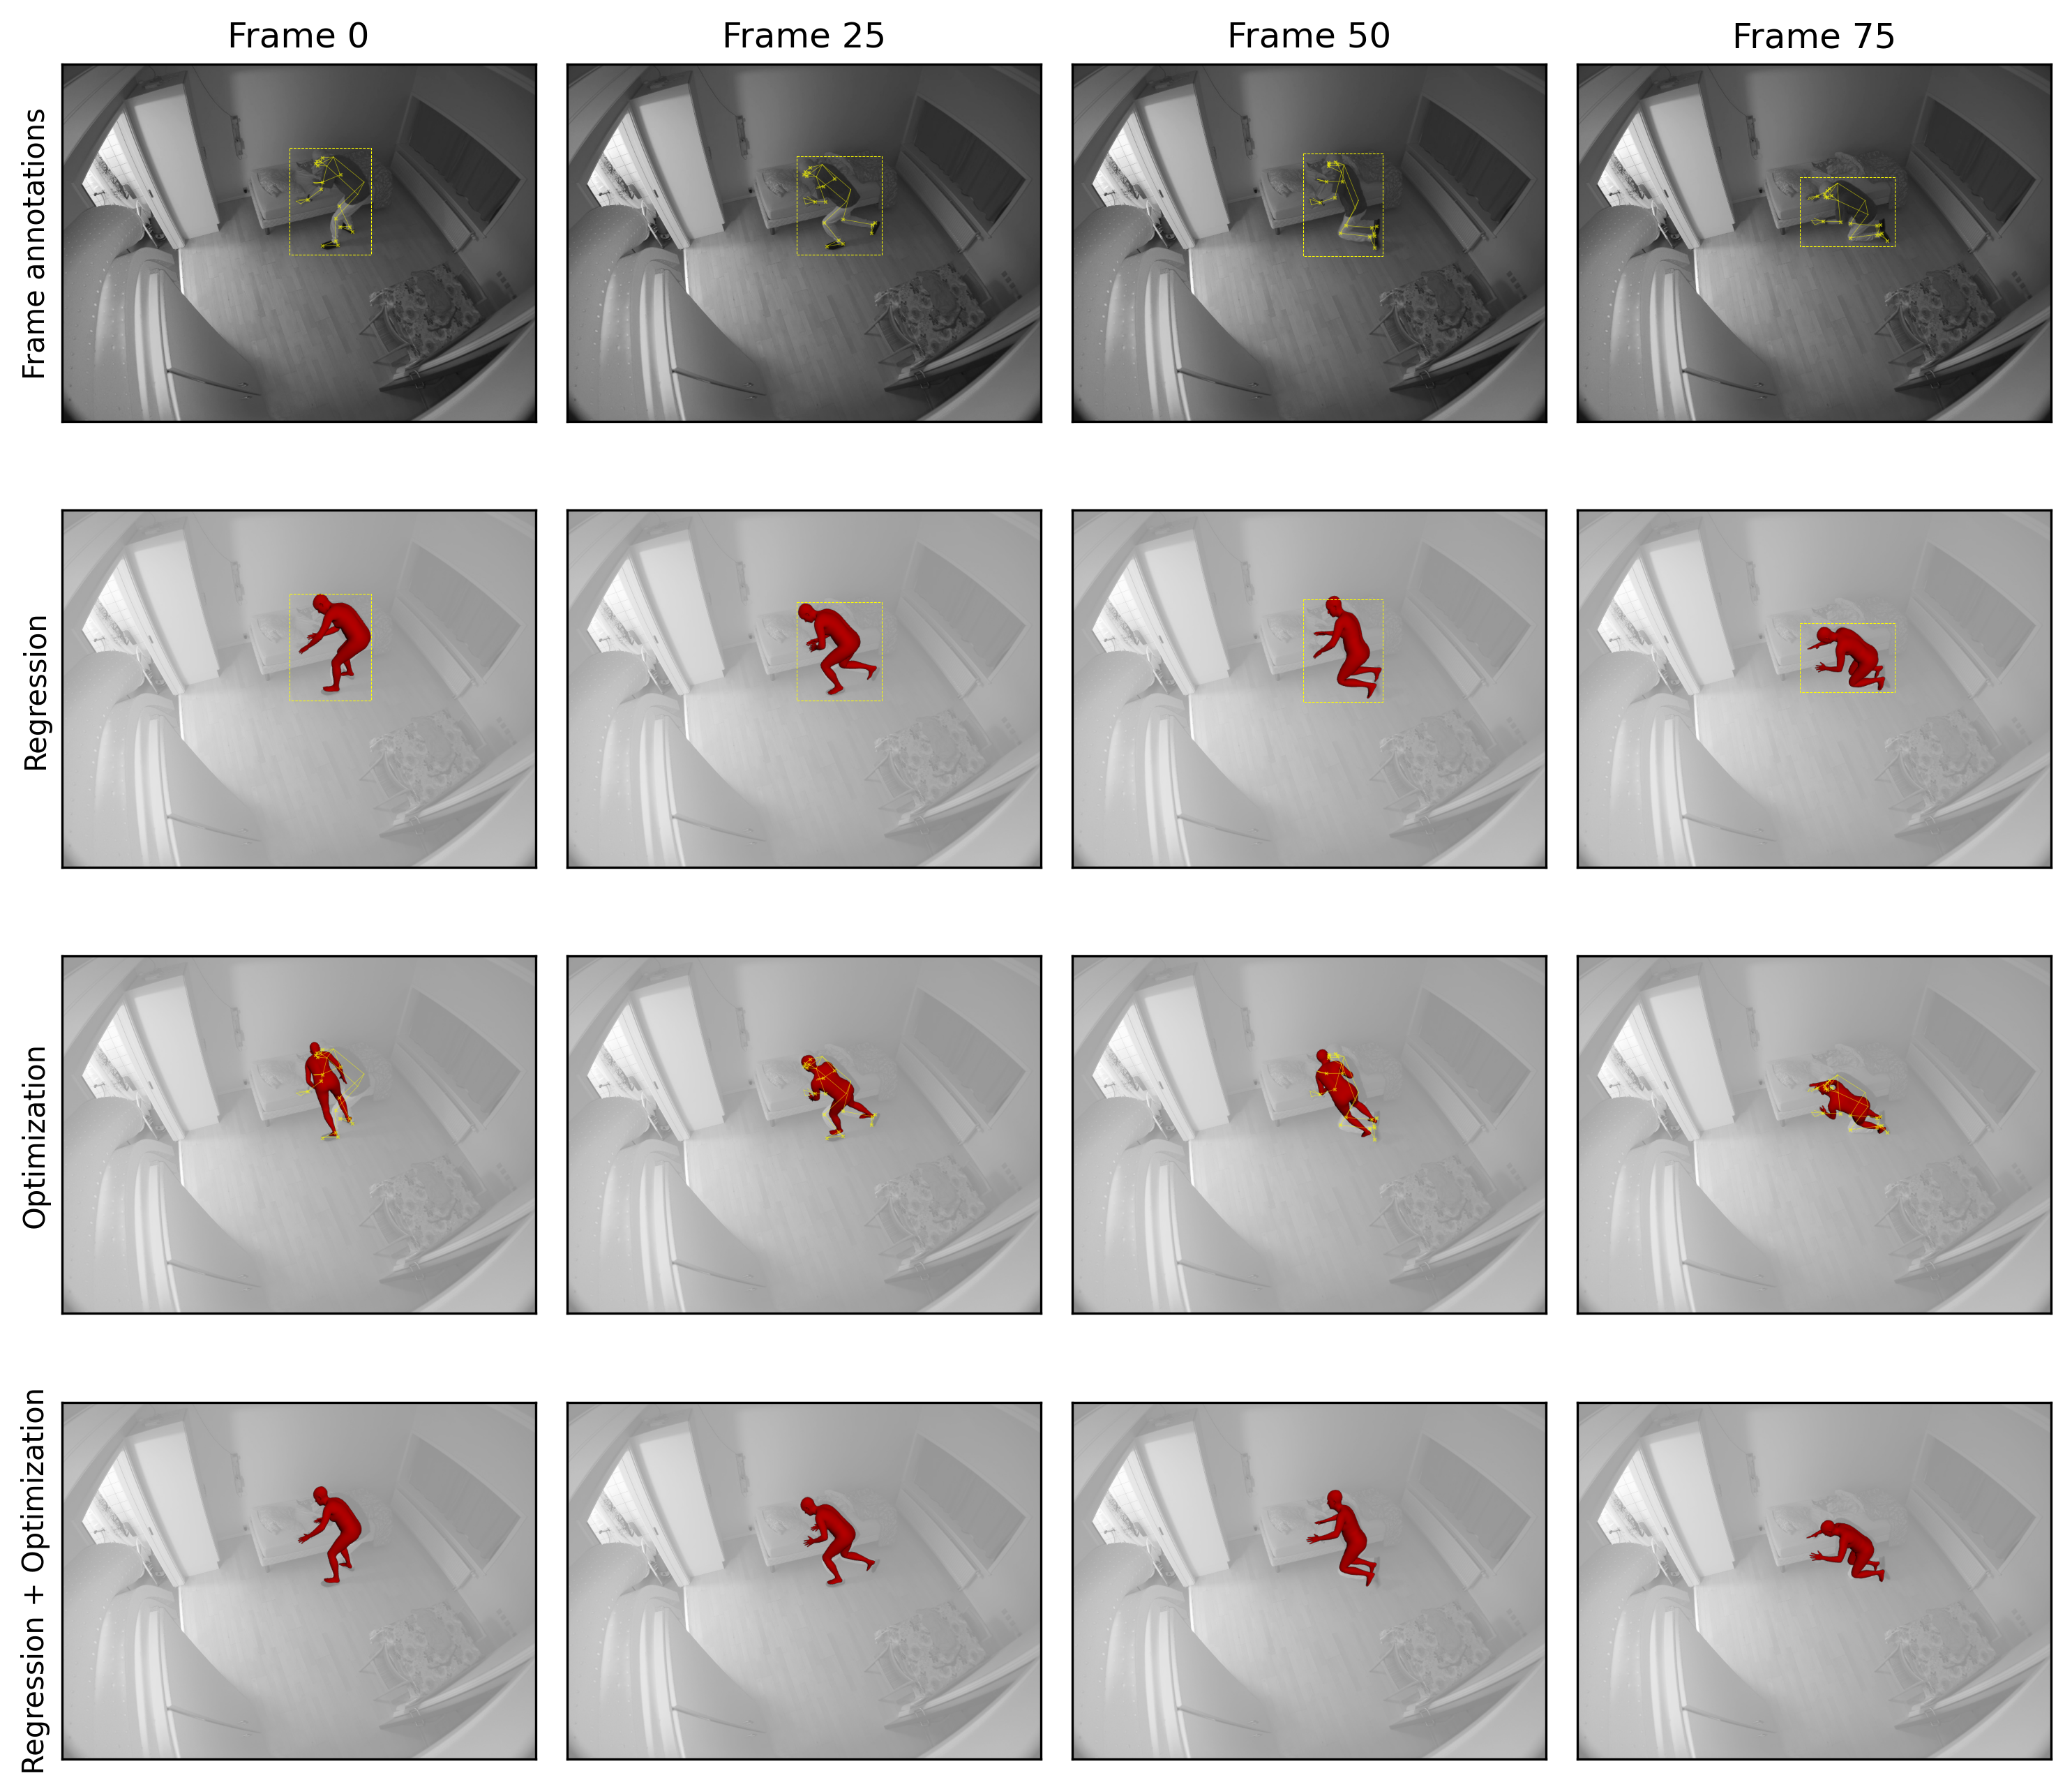
\includegraphics[width=\linewidth]{figures/results/motion2.png}
    \caption{Local optimum of optimization-based method and hybrid method.}
    \label{fig:motion2}
\end{figure}

\begin{figure}
    \centering
    \includegraphics[width=\linewidth]{figures/results/motion3.png}
    \caption{Interpenetration between different people.}
    \label{fig:motion3}
\end{figure}

In the example shown in \cref{fig:motion1}, we notice that the keypoints do not correspond to the actual joints of the person. Specifically, the leg keypoints appear to be incorrectly marked as if the legs were covered by a blanket, despite being visible in the image, as indicated by the red ring. This might be an error in the keypoint annotations, either due to the autolabelling step in the pipeline failing to correctly detect the keypoints or a lack of human attention. As a result, the optimized pose (red) diverges from the actual pose of the person, while the green person's pose looks consistent with the person in the frame. Interestingly, the regressed pose also estimates the legs as being covered by the blanket, although it predicts the pose directly from the image. This again seems to be a result of a bad bounding box segmentation, not including the legs.

A common encountered problem with the optimization-based method is seen in \cref{fig:motion2}, where the optimized pose appears to be stuck in a local optimum during the optimization phase. In contrast, the regression-based method seems to correctly predict the pose but either overestimates the size of the person or places the person too close to the camera. Inspecting the outline of the person in the first frame indicates that the regression-based method might be sensitive to clothing or body shape. Initializing the pose from the regression estimates and then optimizing against the keypoints seems to give the best pose fit. 

As each pose is optimized in isolation, artifacts such as interpenetration might occur, as observed in the last row of \cref{fig:motion3}, after optimizing the initial regression-based estimate to align with the keypoints. Furthermore, the regression-based method fails to detect the occluded nurse behind the bed, as indicated by the semi-transparent mesh, indicating that the pose was removed due to closer matching the keypoints of the laying patient (see \cref{section:regression-pose-estimation}).

% \begin{figure}[H]
%     \centering
%     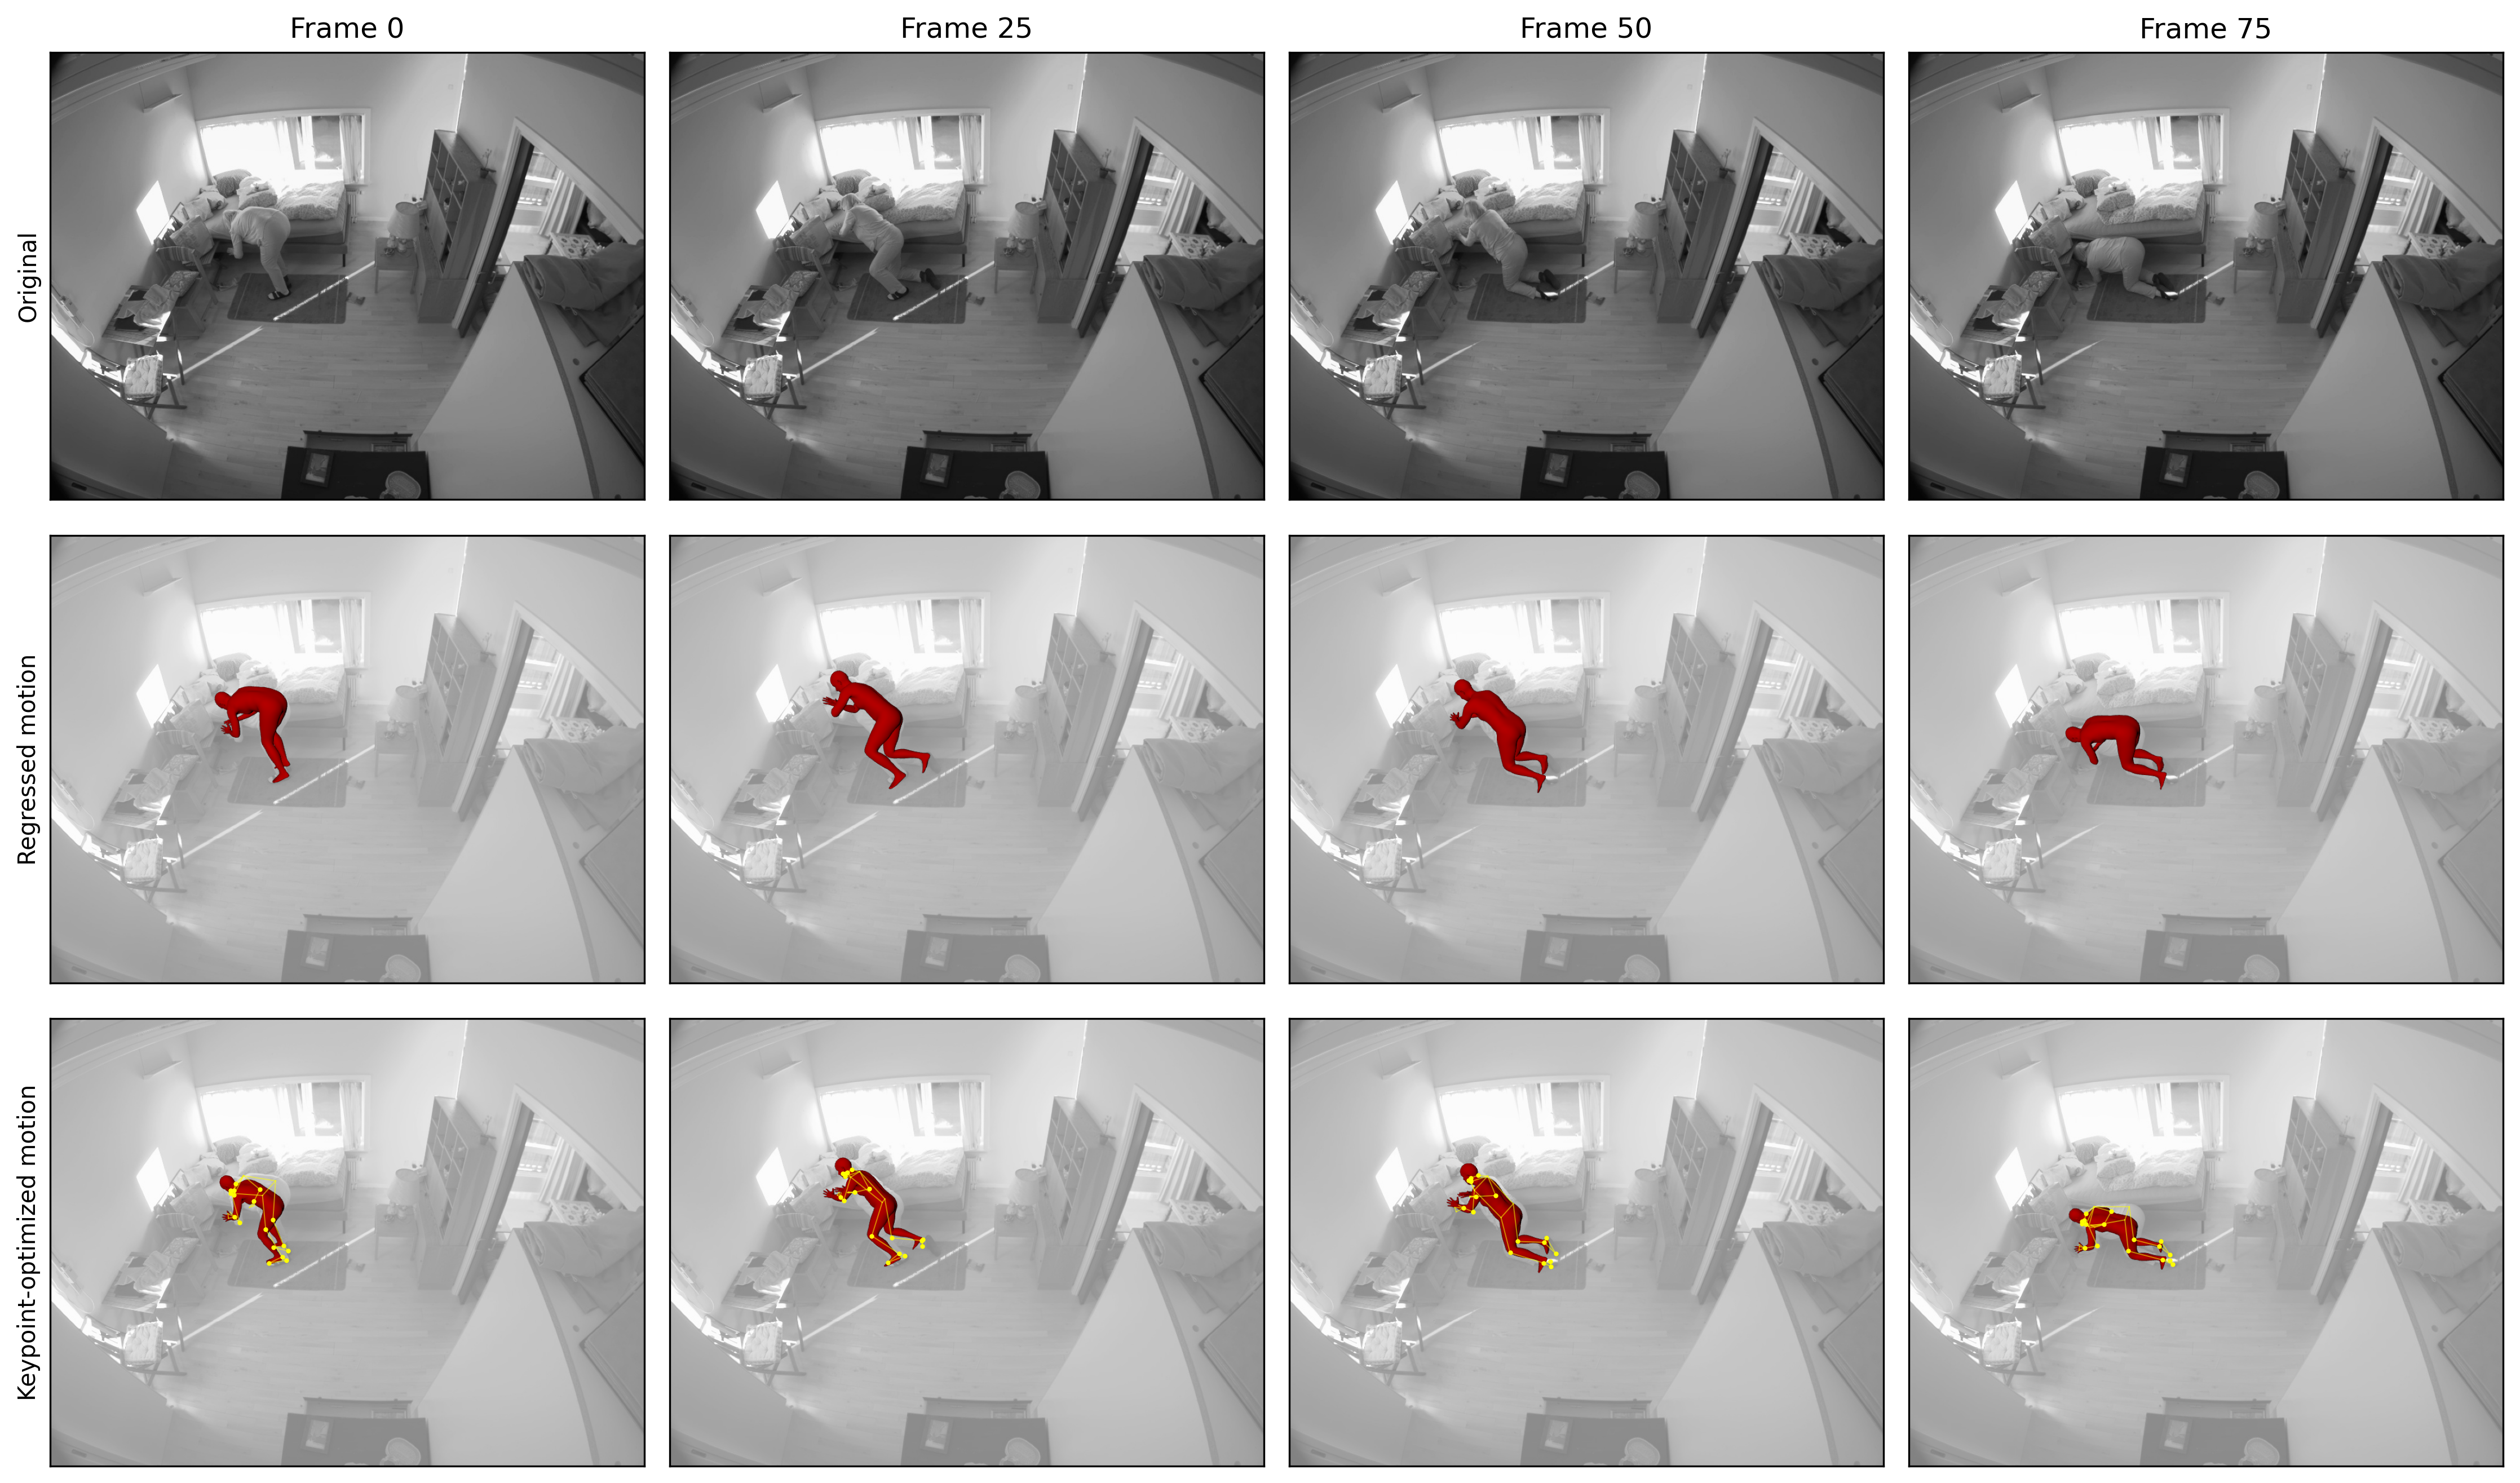
\includegraphics[width=\linewidth]{figures/results/motion4.png}
%     \caption{Example of bad ground truth kpts.}
% \end{figure}

% \begin{figure}[H]
%     \centering
%     \includegraphics[width=\linewidth]{figures/results/motion5.png}
%     \caption{Example of bad ground truth kpts.}
% \end{figure}

\section*{Single-Human Motion Generation}

\begin{figure}
    \centering
    \begin{subfigure}{0.32\linewidth}
        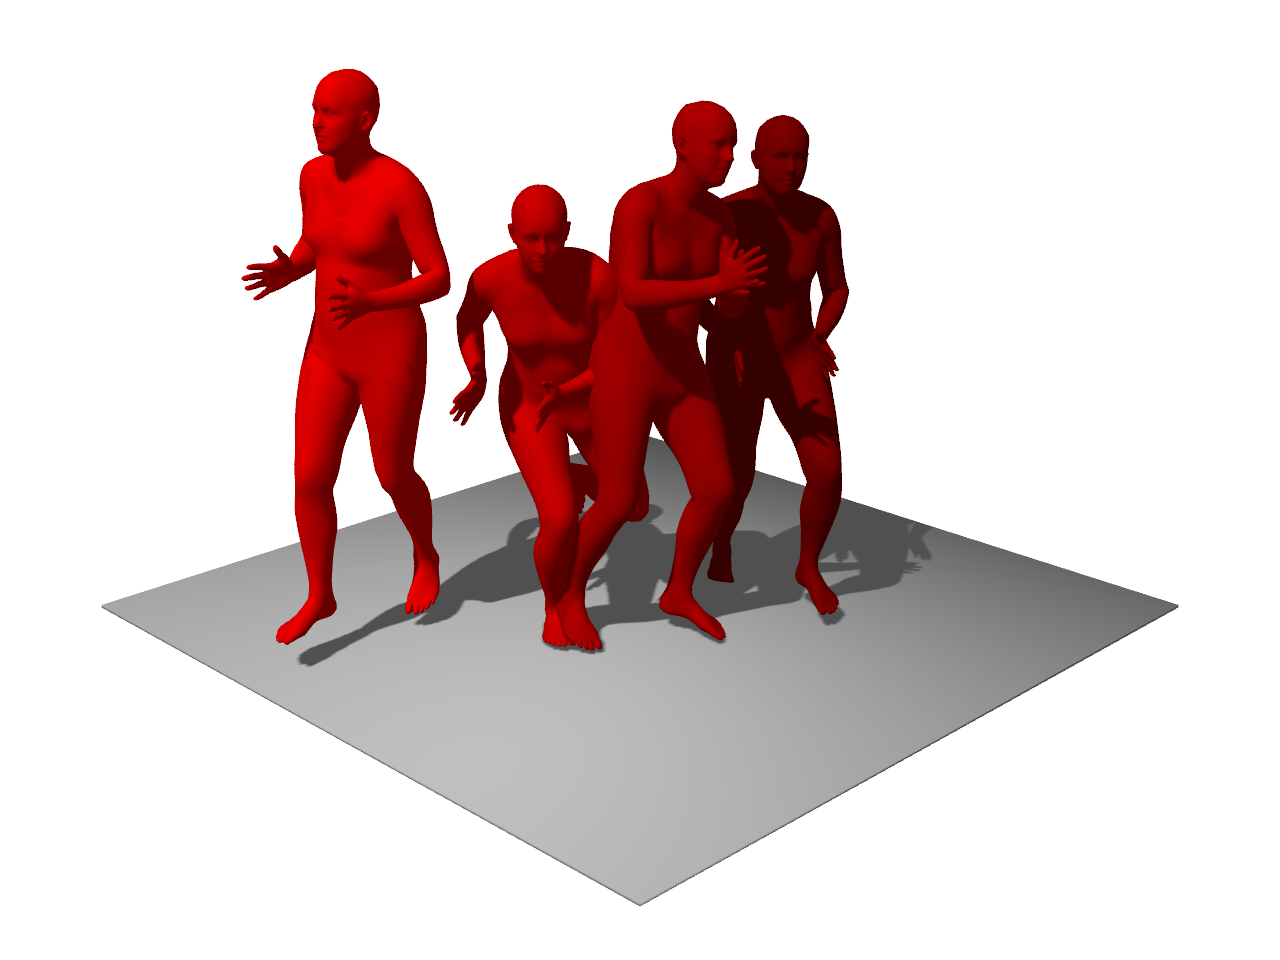
\includegraphics[width=\linewidth]{figures/results/single-kick1.png}
    \end{subfigure}
    \hfill
    \begin{subfigure}{0.32\linewidth}
        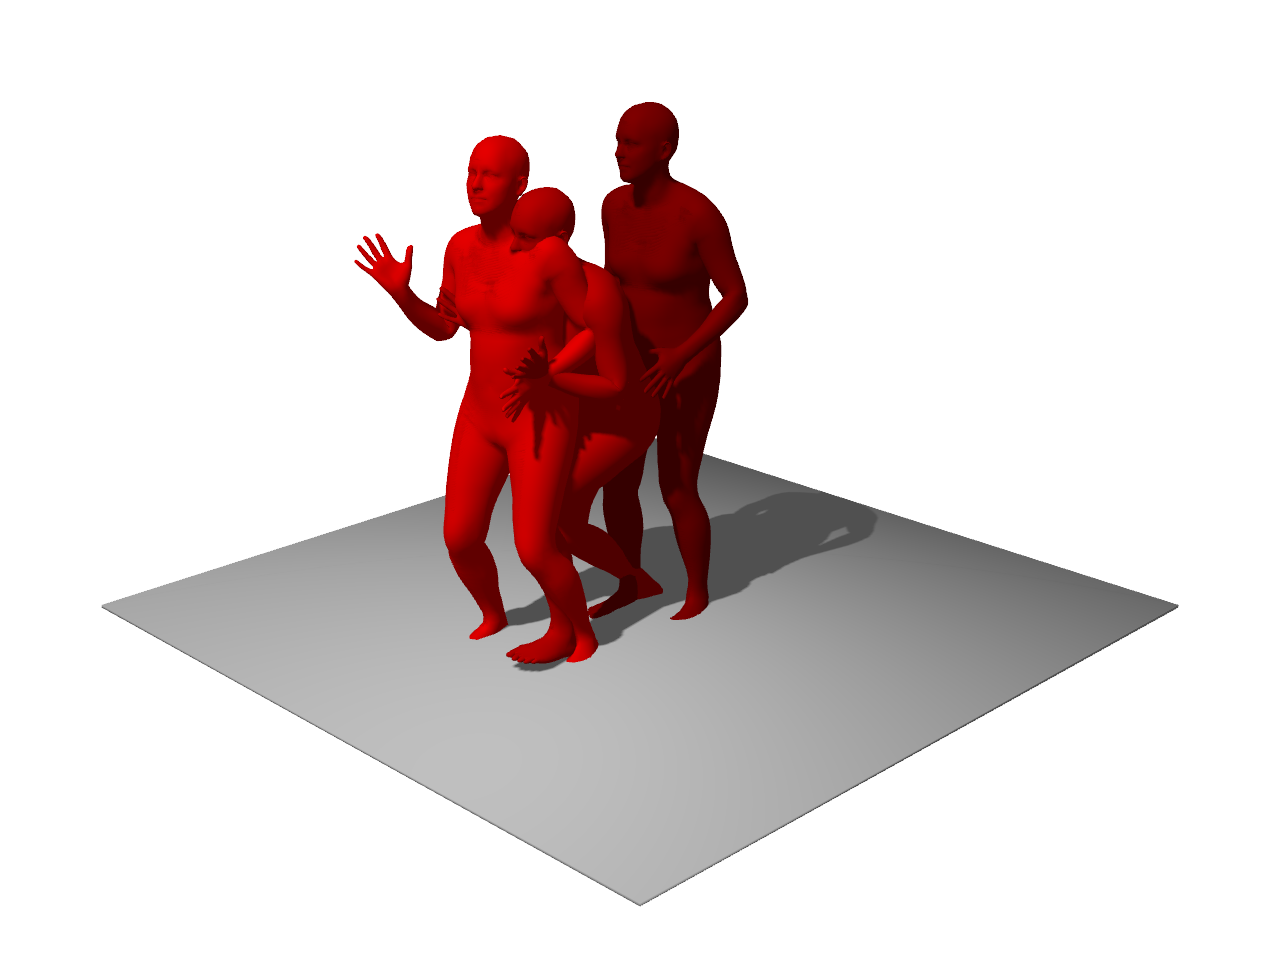
\includegraphics[width=\linewidth]{figures/results/single-kick2.png}
    \end{subfigure}
    \hfill
    \begin{subfigure}{0.32\linewidth}
        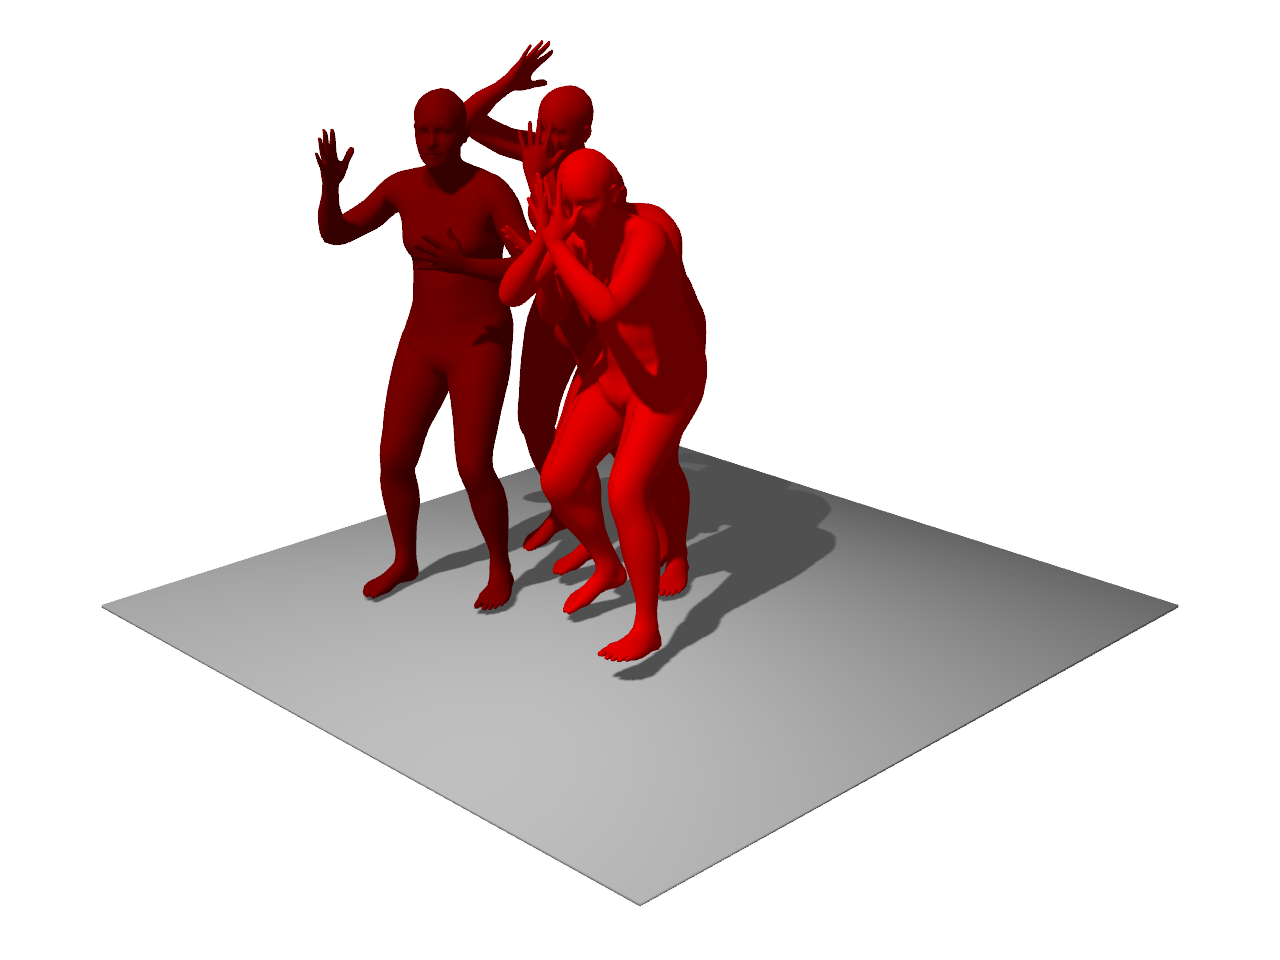
\includegraphics[width=\linewidth]{figures/results/single-kick3.png}
    \end{subfigure}
    \caption{Three examples of single motion generation with prompt: \textit{"A person kicks with their left leg."}}
\end{figure}

\begin{figure}
    \centering
    \begin{subfigure}{0.32\linewidth}
        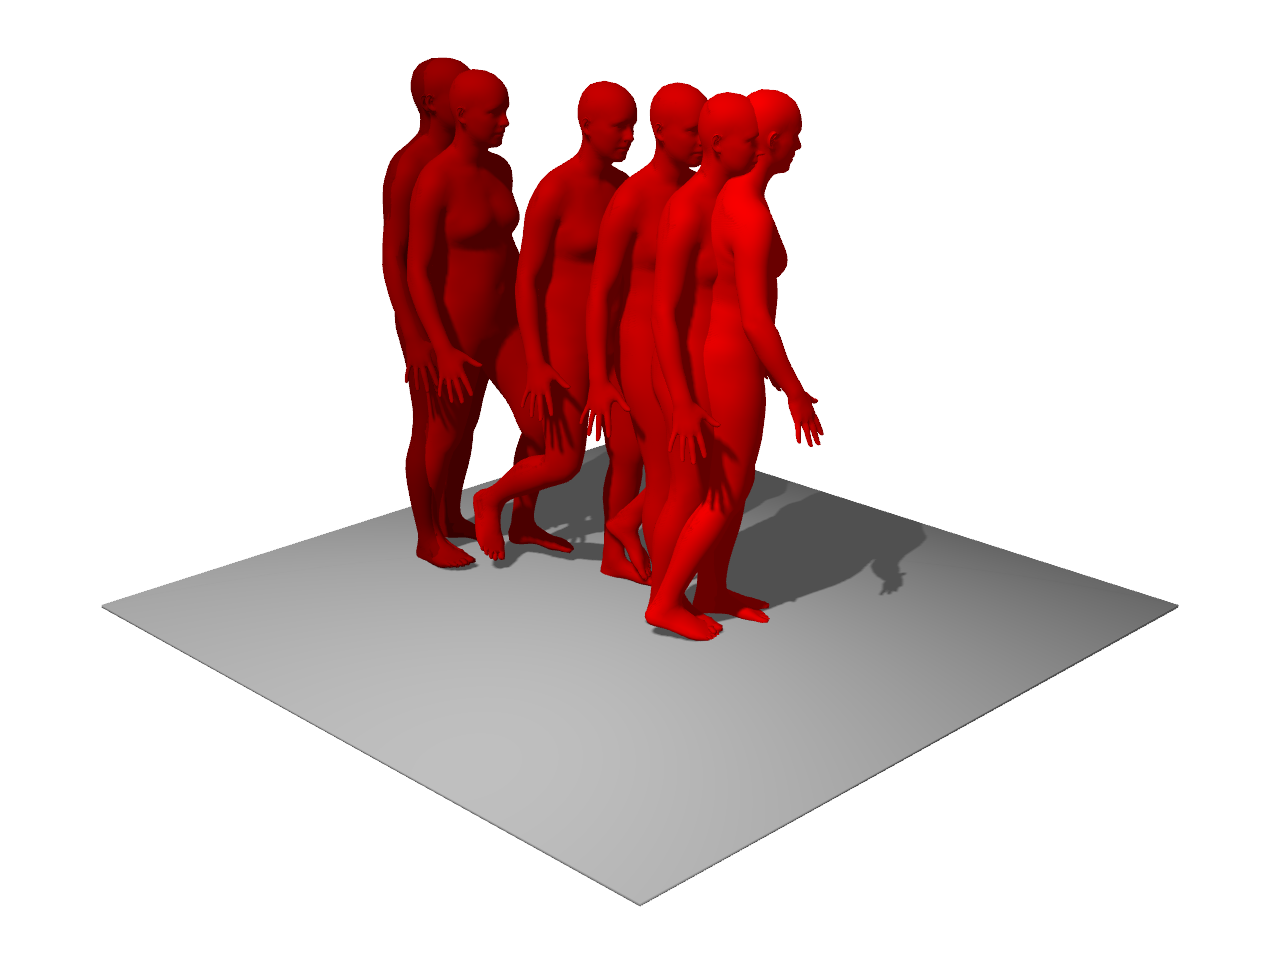
\includegraphics[width=\linewidth]{figures/results/single-runs1.png}
    \end{subfigure}
    \hfill
    \begin{subfigure}{0.32\linewidth}
        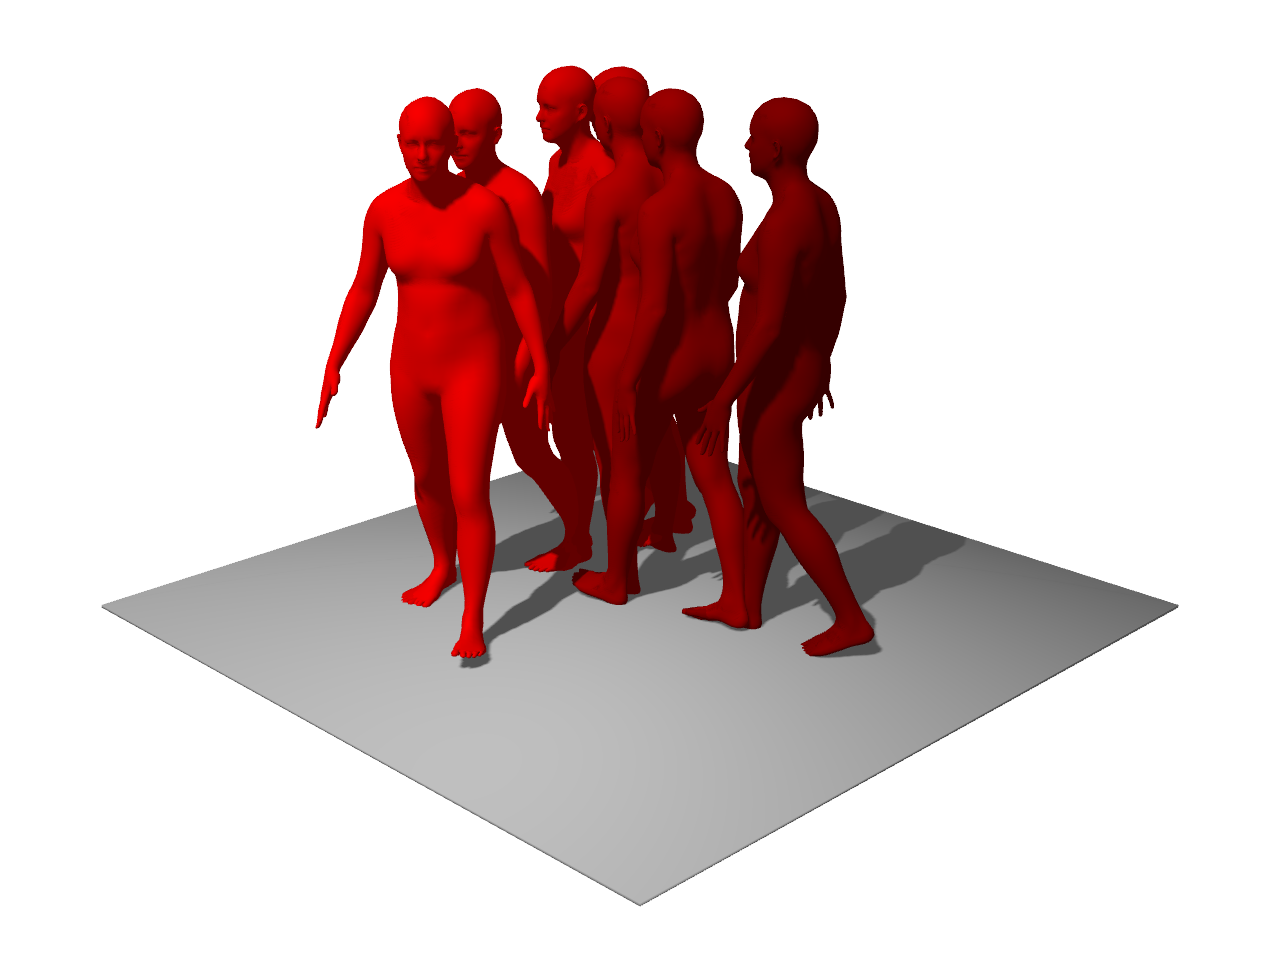
\includegraphics[width=\linewidth]{figures/results/single-runs2.png}
    \end{subfigure}
    \hfill
    \begin{subfigure}{0.32\linewidth}
        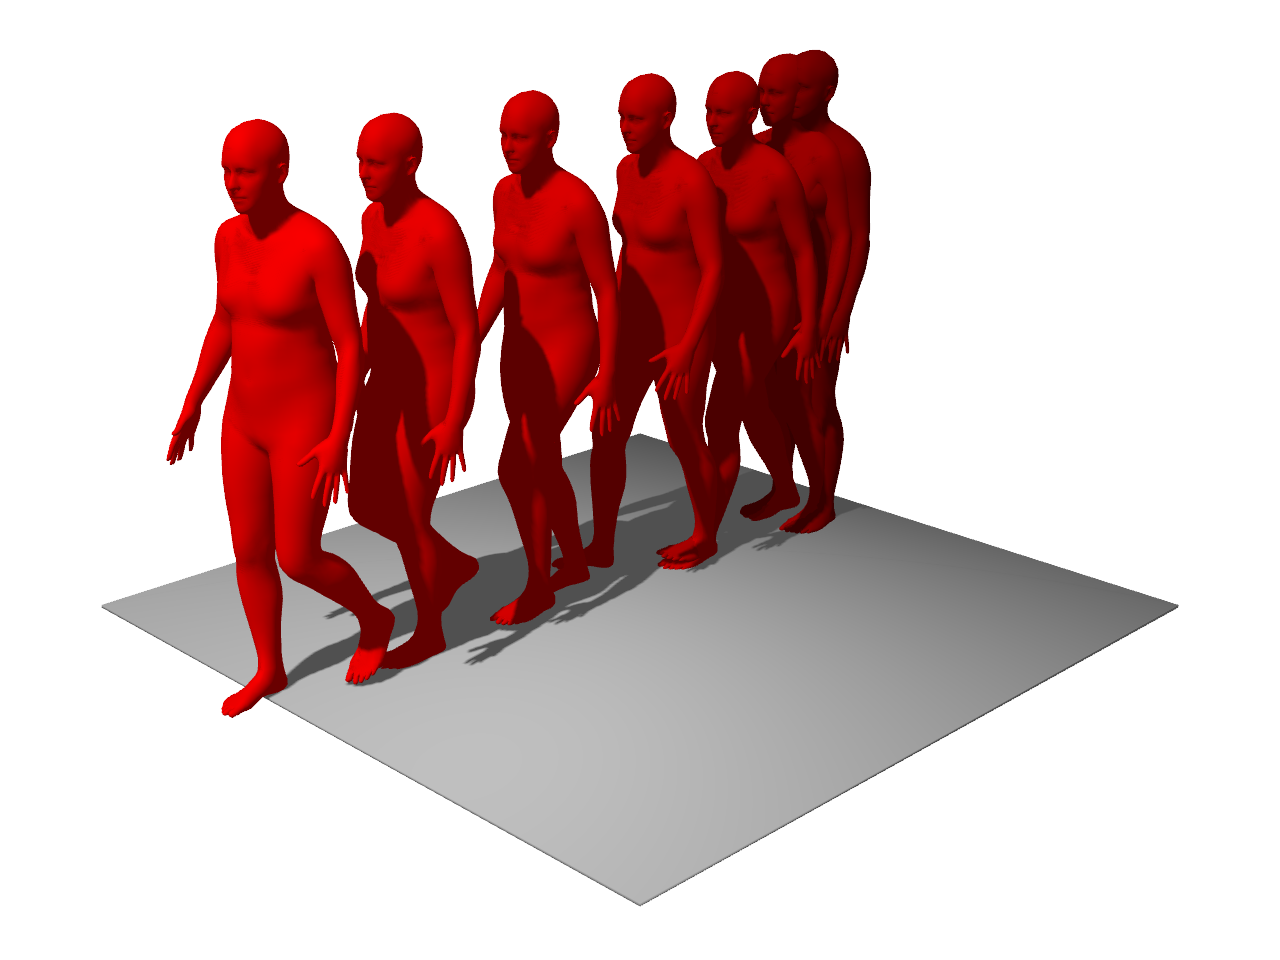
\includegraphics[width=\linewidth]{figures/results/single-runs3.png}
    \end{subfigure}
    \caption{Three randomly picked examples of generated motion with prompt: \textit{"A man runs to the right then runs to the left then back to the middle."}}
\end{figure}


\begin{figure}
    \centering
    \begin{subfigure}{0.32\linewidth}
        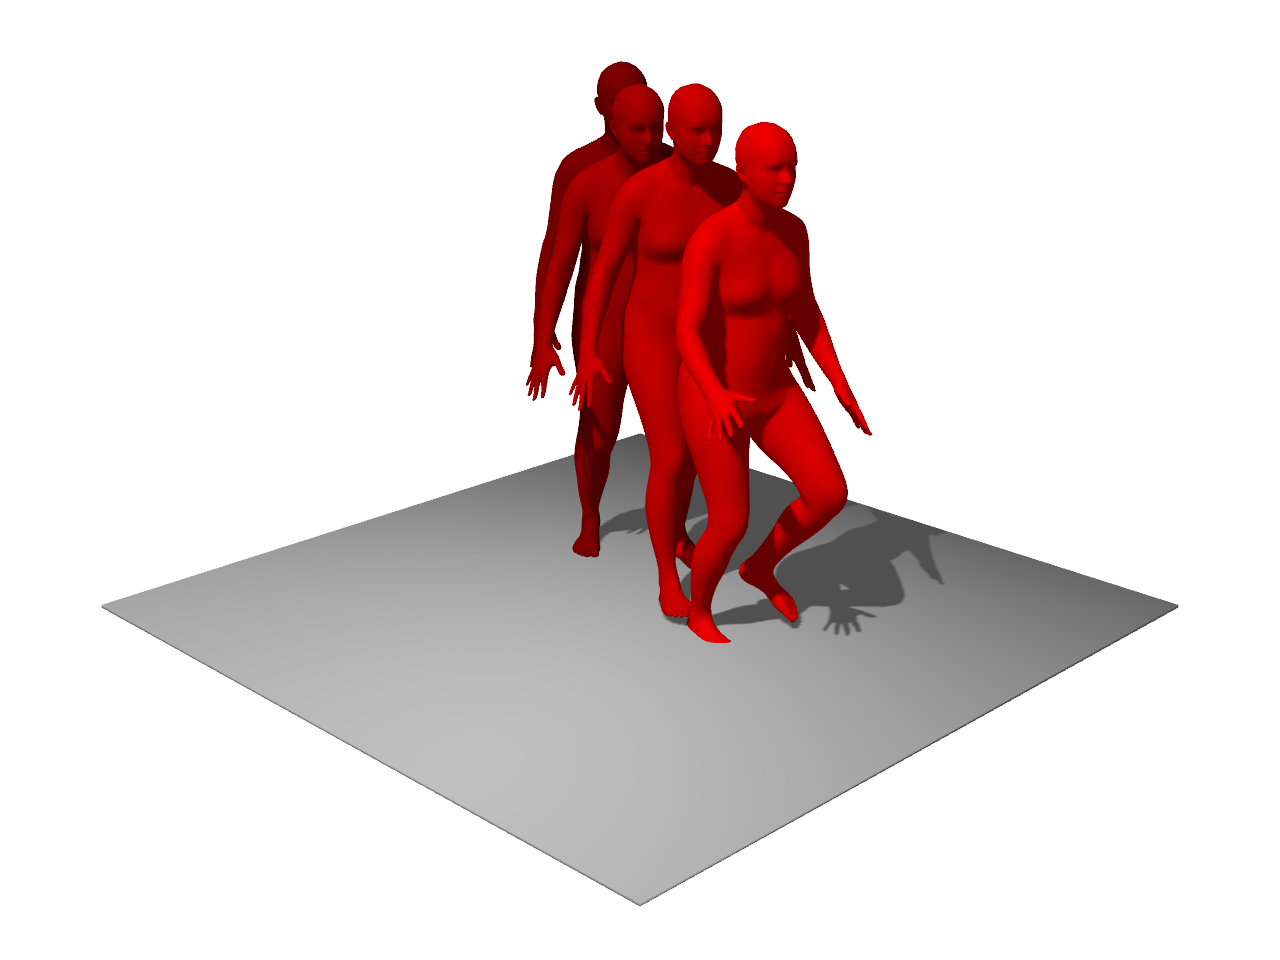
\includegraphics[width=\linewidth]{figures/results/single-falls1.png}
    \end{subfigure}
    \hfill
    \begin{subfigure}{0.32\linewidth}
        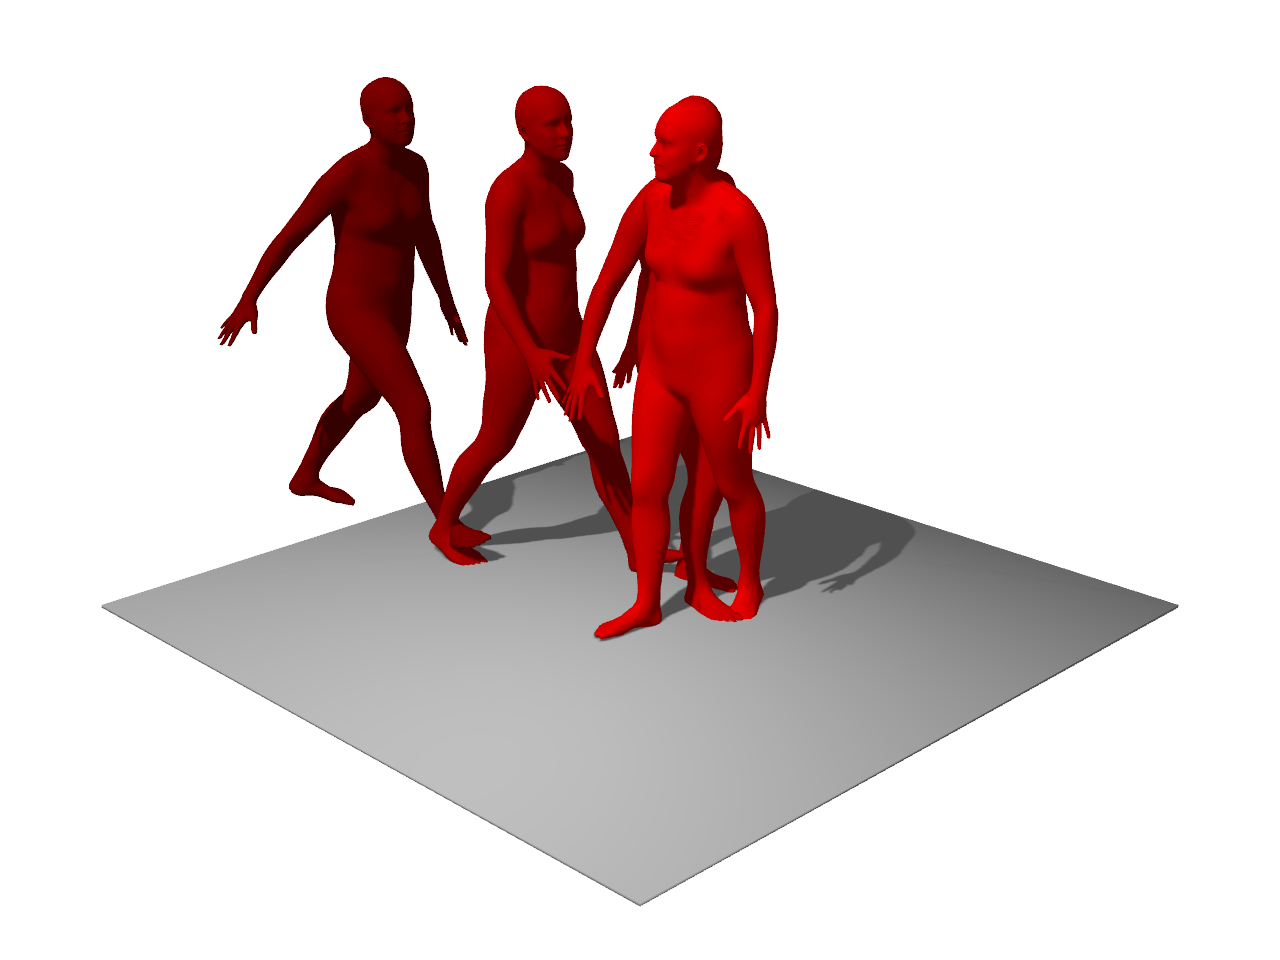
\includegraphics[width=\linewidth]{figures/results/single-falls2.png}
    \end{subfigure}
    \hfill
    \begin{subfigure}{0.32\linewidth}
        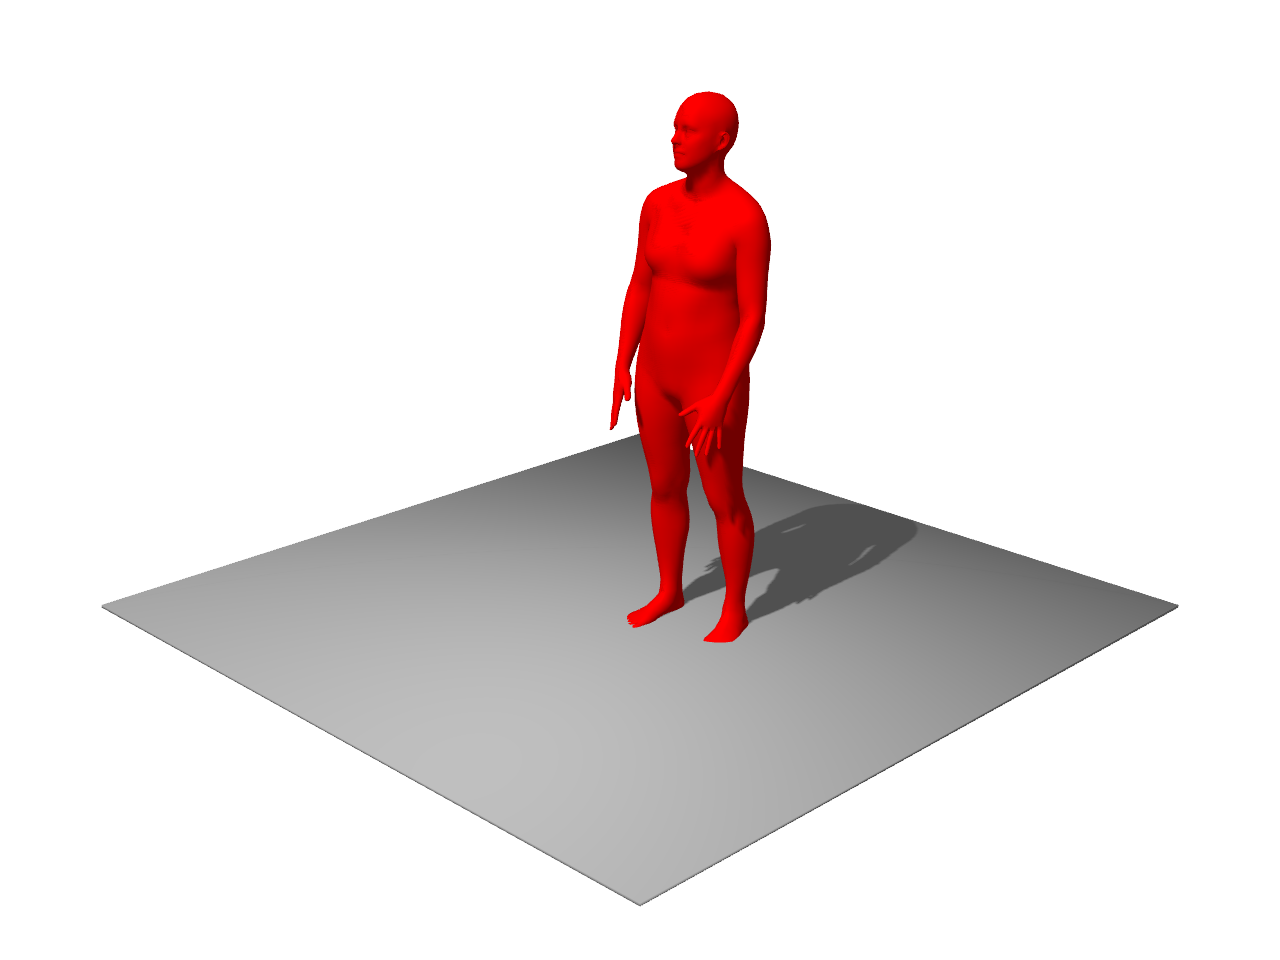
\includegraphics[width=\linewidth]{figures/results/single-falls3.png}
    \end{subfigure}
    \caption{Three randomly picked examples of generated motion with prompt: \textit{"A persons loses balance and falls to the ground."}}
\end{figure}

\section*{Multi-Human Motion Generation}

\begin{figure}
    \centering
    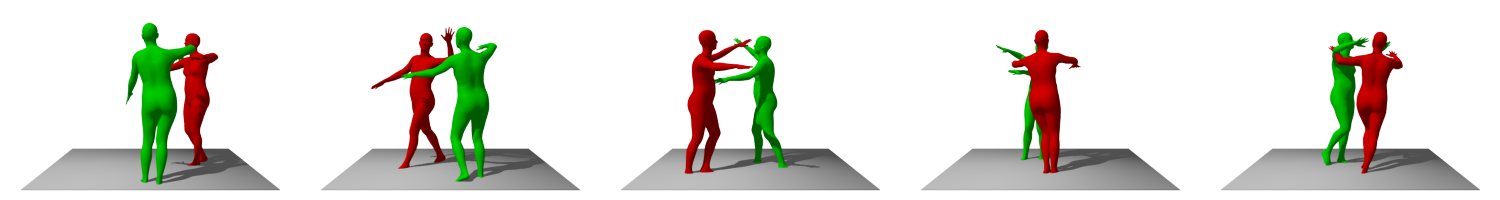
\includegraphics[width=\linewidth]{figures/results/multi-passion.png}
    \caption{Prompt: \textit{"With fiery passion two dancers entwine in Latin dance sublime."}}
\end{figure}


\begin{figure}
    \centering
    \includegraphics[width=\linewidth]{figures/results/multi-selfie1.png}
    \caption{Prompt: \textit{"With merry smiles the two snap their selfie."}}
\end{figure}


\begin{figure}
    \centering
    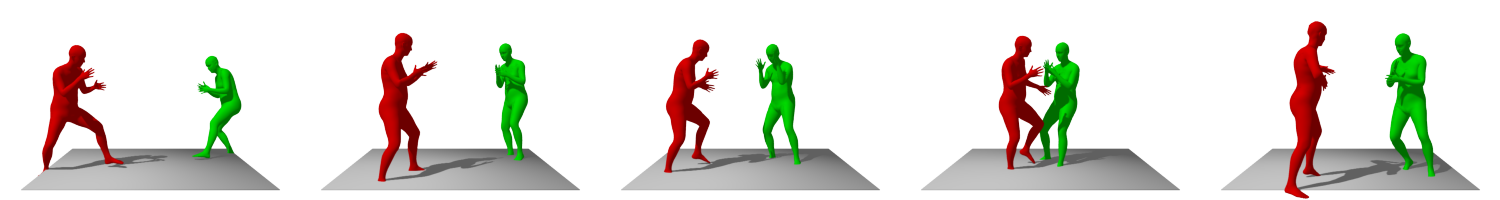
\includegraphics[width=\linewidth]{figures/results/multi-pick-up.png}
    \caption{Prompt: \textit{"Two people picking up something from the ground."}}
\end{figure}
\cleardoublepage 
\chapter{Discussion}

We demonstrate qualitatively good results in reconstructing the 3D environment using current state-of-the-art monocular metric depth estimation models, suggesting the feasibility of this method. However, more careful evaluation is needed, such as benchmarking the estimated depths against actual room scans in the hospital and care home domain.

In motion estimation, we find that the regression-based method, which operates on image bounding boxes, yields the most robust pose estimations. On the other hand, the optimization-based approach provides the most accurate results but is sensitive to poor keypoint annotations. We also test a hybrid method, optimizing an initially regressed pose against the keypoint annotations, to strike a good balance. If time had allowed, it would be interesting to further compare the results with temporal methods such as VIBE (\cite{kocabas2019vibe}) or HuMoR (\cite{rempe2021humor}). 

From our motion generation results, we notice a general pattern of the motion not adhering to the given prompt for many examples, though still generating plausible and realistic motion. This suggests that the model hasn't fully learned the relationship between the prompts and the resulting motions. This issue might be resolved with increased training time, as the tested model was not fully converged due to limited time.

The model might also be overfitting to the data, learning to output the memorized motion closest to the noisy input. This could be a side effect of predicting the signal instead of the noise, making it easier for the model to ignore the input. Predicting the noise instead of the signal might help prevent overfitting, as the noisy input would need to be propagated through the network before being subtracted from the memorized signal to correctly predict the residual noise. Other preventative measures include data augmentation. We initially experimented with applying random rotations and translations but refrained from doing so to more closely reproduce the results of MDM and InterGen. We also performed experiments repurposing an unconditional motion diffusion model for motion estimation, guided by a keypoint loss function, but did not succeed. However, we consistently observed that when applying classifier guidance, the keypoint loss would decrease during the first three-quarters of the denoising process, only to sharply increase afterward. This further supports our belief that the model is overfitting in the later denoising stages.

Although the model is theoretically capable of generating interactive motion for more than two people, in practice, we observe several critical flaws. For instance, poses often collapse or merge, occupying the same space. This conflicts with the purpose of introducing identity encoding, which should help the model differentiate between individuals. One explanation for this issue is that the model has simply learned to differentiate people by their joint positions, ignoring the identity encoding. To validate the effectiveness and usefulness of identity encoding, it may be necessary to train the model on more crowded motions, where such encoding would become more beneficial.

To properly evaluate the motion generation quality and diversity for comparisons with other methods, quantative metrics such as the Fréchet Inception Distance (FID), Diversity and Multimodality metrics as introduced by \cite{Guo_2020} are typically reported. However, due to incompatibility of the code, requiring extensive modifications, this became infeasible within the last phase of the thesis.


\chapter{Conclusion}
In conclusion, we compared different methods for restoring 3D scenes from 2D videos of hospital and care-home scenarios. We divided the problem into two parts: 3D reconstruction of the environment and restoration of human motion using both regression-based and optimization-based methods. Additionally, we demonstrated how diffusion models can be trained to generate realistic human motion and extended the InterGen model to generate interactions among a variable number of humans. We found that our model is likely overfitting and that the generated motions generally fail to adhere to the given prompts. We also suggested several measures to address these issues. Further quantitative evaluation is needed to conclusively determine the effectiveness of all three methods. 
\cleardoublepage 
%%%%%%%%%%%%%%%%%%%%%%%%%%%%%%%%%%%%%%%%%%%%%%%%%%%%%%%
\printbibliography[heading=bibintoc,title={Bibliography}]
\cleardoublepage 
\appendix
\chapter{Appendices}

\section{Derivation of posterior distribution} \label{appendix:q-posterior-derivation}
\begin{align*}
    q(\mathbf{x}_{t-1} \vert \mathbf{x}_t, \mathbf{x}_0) &= q(\mathbf{x}_t \vert \mathbf{x}_{t-1}, \mathbf{x}_0) \frac{q(\mathbf{x}_{t-1} \vert \mathbf{x}_0)}{q(\mathbf{x}_t \vert \mathbf{x}_0)} \\
    \Leftrightarrow \log q(\mathbf{x}_{t-1} \vert \mathbf{x}_t, \mathbf{x}_0) &= \log q(\mathbf{x}_t \vert \mathbf{x}_{t-1}, \mathbf{x}_0) + 
    \log q(\mathbf{x}_{t-1} \vert \mathbf{x}_0) - \log q(\mathbf{x}_t \vert \mathbf{x}_0) \\
    &= \frac{1}{2} \left( 
        \frac{\left( \mathbf{x}_t - \sqrt{\alpha_t} \mathbf{x}_{t-1} \right)^2}{\beta_t} +
        \frac{\left( \mathbf{x}_{t-1} - \sqrt{\bar{\alpha}_{t-1}} \mathbf{x}_0 \right)^2}{1 - \bar{\alpha}_{t-1}} + 
        \frac{\left( \mathbf{x}_{t} - \sqrt{\bar{\alpha}_{t}} \mathbf{x}_0 \right)^2}{1 - \bar{\alpha}_{t}}
    \right) + K \\
    &= \frac{1}{2} \left(
        \frac{\mathbf{x}_t^2 - 2 \sqrt{\alpha_t}\mathbf{x}_t \mathbf{x}_{t-1} + \alpha_t \mathbf{x}_{t-1}^2}{\beta_t} +
        \frac{\mathbf{x}_{t-1}^2 - 2  \sqrt{\bar{\alpha}_{t-1}} \mathbf{x}_{t-1} \mathbf{x}_0 + \bar{\alpha}_{t-1}\mathbf{x}_0^2  }{1 - \bar{\alpha}_{t-1}} + C(x_t, x_0)
    \right) + K
\end{align*}

We collect all terms for $\mathbf{x}_{t-1}$ and $\mathbf{x}_{t-1}^2$. 

\cleartoleftpage
\newgeometry{left=28mm,right=14mm,top=42mm,bottom=14mm}
\thispagestyle{empty}
\pagecolor{frontbackcolor}
\color{white}

%\blindtext % Remove this for a blank page or write your own text

\vspace*{\fill}



\begin{tabular}{@{}l}
    Technical \\ 
    University of \\ 
    Denmark \\
    \\
    \addressI \\
    \addressII \\
    Tlf. 4525 1700 \\
    \\
    \url{\departmentwebsite}
\end{tabular}



\end{document}